\documentclass{article}
\usepackage{geometry}
\usepackage{amsmath}
\usepackage{lscape}
\geometry{verbose,tmargin=2.5cm,bmargin=2.5cm,lmargin=2.5cm,rmargin=2.5cm}

\begin{document}



\title{NSWPCN Predictor Training}
\maketitle

%%%%%%%%%%%%%%%%%%%%%%%%%%%%%%%%%%%%%%%%%%%%%%%%%%%%%%%%%%%%%%%%%%%%%%
% LIBRARIES
%%%%%%%%%%%%%%%%%%%%%%%%%%%%%%%%%%%%%%%%%%%%%%%%%%%%%%%%%%%%%%%%%%%%%%
\section{Preparation}
\begin{knitrout}
\definecolor{shadecolor}{rgb}{0.969, 0.969, 0.969}\color{fgcolor}\begin{kframe}
\begin{alltt}
\hlkwd{library}\hlstd{(survival)}
\hlkwd{library}\hlstd{(glmulti)}
\hlkwd{library}\hlstd{(flexsurv)}
\hlkwd{library}\hlstd{(randomForestSRC)}

\hlkwd{library}\hlstd{(reshape2)}
\hlkwd{library}\hlstd{(plyr)}
\hlkwd{library}\hlstd{(ggplot2)}

\hlkwd{library}\hlstd{(MASS)}
\hlkwd{library}\hlstd{(boot)}
\hlkwd{library}\hlstd{(timeROC)}

\hlkwd{load}\hlstd{(}\hlstr{"03_NSWPCN_subset.rda"}\hlstd{)}
\end{alltt}
\end{kframe}
\end{knitrout}


%%%%%%%%%%%%%%%%%%%%%%%%%%%%%%%%%%%%%%%%%%%%%%%%%%%%%%%%%%%%%%%%%%%%%%
% DATA SELECTION
%%%%%%%%%%%%%%%%%%%%%%%%%%%%%%%%%%%%%%%%%%%%%%%%%%%%%%%%%%%%%%%%%%%%%%
\section{Cohort selection and transformation}
\begin{knitrout}
\definecolor{shadecolor}{rgb}{0.969, 0.969, 0.969}\color{fgcolor}\begin{kframe}
\begin{alltt}
\hlstd{x} \hlkwb{=} \hlstd{data[,}\hlkwd{c}\hlstd{(}\hlstr{"Patient.Sex"}\hlstd{,} \hlstr{"History.Diagnosis.AgeAt.Cent"}\hlstd{,} \hlstr{"Path.LocationBody"}\hlstd{,} \hlstr{"Path.Size.Cent"}\hlstd{,} \hlstr{"Path.Ca199.Preop"}\hlstd{,} \hlstr{"Molec.S100A2.DCThresh"}\hlstd{,} \hlstr{"Molec.S100A4.DCThresh"}\hlstd{)]}
\hlkwd{colnames}\hlstd{(x)} \hlkwb{=} \hlkwd{c}\hlstd{(}\hlstr{"SexM"}\hlstd{,} \hlstr{"AgeCent"}\hlstd{,} \hlstr{"LocBody"}\hlstd{,} \hlstr{"SizeCent"}\hlstd{,} \hlstr{"Ca199"}\hlstd{,} \hlstr{"A2"}\hlstd{,} \hlstr{"A4"}\hlstd{)}
\hlstd{x}\hlopt{$}\hlstd{SexM} \hlkwb{=} \hlstd{x}\hlopt{$}\hlstd{Sex} \hlopt{==} \hlstr{"M"}
\hlstd{x}\hlopt{$}\hlstd{Ca199} \hlkwb{=} \hlstd{x}\hlopt{$}\hlstd{Ca199} \hlopt{>} \hlnum{100}

\hlstd{y} \hlkwb{=} \hlkwd{Surv}\hlstd{(}\hlkwd{as.numeric}\hlstd{(data}\hlopt{$}\hlstd{History.Death.Date} \hlopt{-} \hlstd{data}\hlopt{$}\hlstd{History.Diagnosis.Date), data}\hlopt{$}\hlstd{History.DSDeath.Event)}
\hlcom{# Note no surgery dates, though for almost all pts there were only a few days difference.}

\hlstd{temp} \hlkwb{=} \hlnum{NA}
\hlstd{temp} \hlkwb{=} \hlkwd{ls}\hlstd{()}
\hlkwd{rm}\hlstd{(}\hlkwc{list} \hlstd{= temp[}\hlopt{!}\hlstd{(temp} \hlopt \hlkwd{c}\hlstd{(}\hlstr{"x"}\hlstd{,} \hlstr{"y"}\hlstd{))])}

\hlstd{sel} \hlkwb{=} \hlopt{!}\hlkwd{is.na}\hlstd{(y[,}\hlnum{1}\hlstd{])} \hlopt{& !}\hlkwd{is.na}\hlstd{(y[,}\hlnum{2}\hlstd{])} \hlopt{& !}\hlkwd{is.na}\hlstd{(x}\hlopt{$}\hlstd{A2)} \hlopt{& !}\hlkwd{is.na}\hlstd{(x}\hlopt{$}\hlstd{A4)} \hlopt{& !}\hlkwd{is.na}\hlstd{(x}\hlopt{$}\hlstd{LocBody)}
\hlstd{x} \hlkwb{=} \hlstd{x[sel,]}
\hlstd{y} \hlkwb{=} \hlstd{y[sel,]}
\hlkwd{rm}\hlstd{(sel)}

\hlcom{# Remove CA-19-9 measurements as they're mostly missing}
\hlstd{x} \hlkwb{=} \hlstd{x[,}\hlkwd{colnames}\hlstd{(x)} \hlopt{!=} \hlstr{"Ca199"}\hlstd{]}

\hlstd{data} \hlkwb{=} \hlkwd{as.data.frame}\hlstd{(}\hlkwd{cbind}\hlstd{(}\hlkwc{Time} \hlstd{= y[,}\hlnum{1}\hlstd{],} \hlkwc{DSD} \hlstd{= y[,}\hlnum{2}\hlstd{], x))}
\hlkwd{rm}\hlstd{(x, y)}
\hlstd{data}\hlopt{$}\hlstd{DSD} \hlkwb{=} \hlstd{data}\hlopt{$}\hlstd{DSD} \hlopt{==} \hlnum{1}
\end{alltt}
\end{kframe}
\end{knitrout}


%%%%%%%%%%%%%%%%%%%%%%%%%%%%%%%%%%%%%%%%%%%%%%%%%%%%%%%%%%%%%%%%%%%%%%
% DATA SPLITTING
%%%%%%%%%%%%%%%%%%%%%%%%%%%%%%%%%%%%%%%%%%%%%%%%%%%%%%%%%%%%%%%%%%%%%%
\section{Data splitting}
There's going to be an awful lot of model manipulation and black magic going on.  Create a holdout validation set for final model comparison and selection.
\begin{knitrout}
\definecolor{shadecolor}{rgb}{0.969, 0.969, 0.969}\color{fgcolor}\begin{kframe}
\begin{alltt}
\hlkwd{set.seed}\hlstd{(}\hlnum{20150110}\hlstd{)}
\hlstd{sel.val} \hlkwb{=} \hlkwd{sample.int}\hlstd{(}\hlkwd{nrow}\hlstd{(data),} \hlkwd{floor}\hlstd{(}\hlkwd{nrow}\hlstd{(data)}\hlopt{/}\hlnum{5}\hlstd{))}
\hlstd{sel.val} \hlkwb{=} \hlnum{1}\hlopt{:}\hlkwd{nrow}\hlstd{(data)} \hlopt \hlstd{sel.val}
\hlkwd{mean}\hlstd{(sel.val)}
\end{alltt}
\begin{verbatim}
## [1] 0.1967
\end{verbatim}
\begin{alltt}
\hlstd{data.val} \hlkwb{=} \hlstd{data[sel.val,,}\hlkwc{drop} \hlstd{=} \hlnum{FALSE}\hlstd{]}
\hlstd{data} \hlkwb{=} \hlstd{data[}\hlopt{!}\hlstd{sel.val,,}\hlkwc{drop} \hlstd{=} \hlnum{FALSE}\hlstd{]}
\end{alltt}
\end{kframe}
\end{knitrout}


%%%%%%%%%%%%%%%%%%%%%%%%%%%%%%%%%%%%%%%%%%%%%%%%%%%%%%%%%%%%%%%%%%%%%%
% MODEL SPECIFICATION
%%%%%%%%%%%%%%%%%%%%%%%%%%%%%%%%%%%%%%%%%%%%%%%%%%%%%%%%%%%%%%%%%%%%%%
\section{EDA}
Use the CPH model as a convenient framework for EDA.
\subsection{Functional form}
Investigate functional form with martingale residuals.
\begin{knitrout}
\definecolor{shadecolor}{rgb}{0.969, 0.969, 0.969}\color{fgcolor}\begin{kframe}
\begin{alltt}
\hlstd{fit.cph.NoAge} \hlkwb{=} \hlkwd{coxph}\hlstd{(}\hlkwd{Surv}\hlstd{(Time, DSD)} \hlopt{~} \hlstd{SexM} \hlopt{+} \hlstd{LocBody} \hlopt{+} \hlstd{SizeCent} \hlopt{+} \hlstd{A2} \hlopt{+} \hlstd{A4,} \hlkwc{data} \hlstd{= data)}
\hlkwd{scatter.smooth}\hlstd{(data}\hlopt{$}\hlstd{AgeCent,} \hlkwd{resid}\hlstd{(fit.cph.NoAge,} \hlkwc{type} \hlstd{=} \hlstr{"martingale"}\hlstd{),} \hlkwc{xlab} \hlstd{=} \hlstr{""}\hlstd{,} \hlkwc{ylab} \hlstd{=} \hlstr{"Martingale residual"}\hlstd{)}
\end{alltt}
\end{kframe}

{\centering 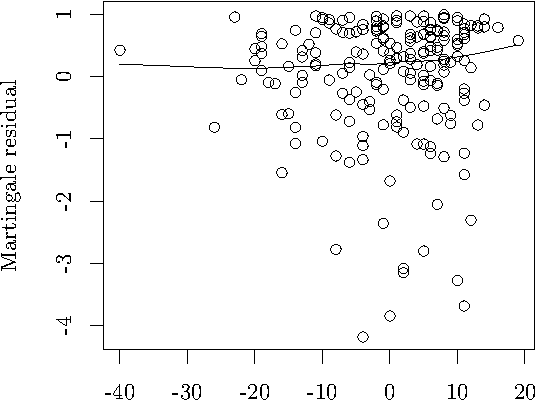
\includegraphics[width=\maxwidth]{figure/05-eda-func-form-age-1} 

}


\begin{kframe}\begin{alltt}
\hlkwd{scatter.smooth}\hlstd{(data}\hlopt{$}\hlstd{AgeCent,} \hlkwd{resid}\hlstd{(fit.cph.NoAge,} \hlkwc{type} \hlstd{=} \hlstr{"martingale"}\hlstd{),} \hlkwc{xlab} \hlstd{=} \hlstr{""}\hlstd{,} \hlkwc{ylab} \hlstd{=} \hlstr{"Martingale residual"}\hlstd{,} \hlkwc{ylim} \hlstd{=} \hlkwd{c}\hlstd{(}\hlopt{-}\hlnum{1}\hlstd{,} \hlnum{1}\hlstd{))}
\end{alltt}
\end{kframe}

{\centering 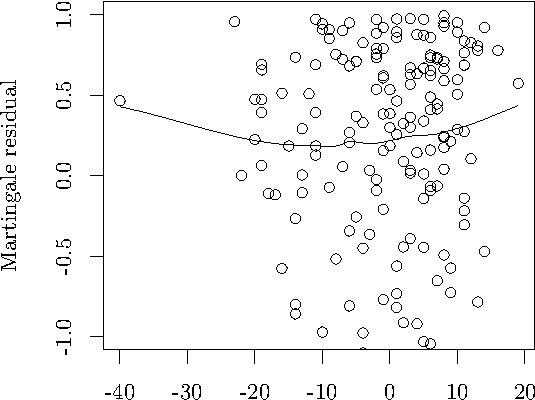
\includegraphics[width=\maxwidth]{figure/05-eda-func-form-age-2} 

}



\end{knitrout}

\begin{knitrout}
\definecolor{shadecolor}{rgb}{0.969, 0.969, 0.969}\color{fgcolor}\begin{kframe}
\begin{alltt}
\hlstd{fit.cph.NoSize} \hlkwb{=} \hlkwd{coxph}\hlstd{(}\hlkwd{Surv}\hlstd{(Time, DSD)} \hlopt{~} \hlstd{SexM} \hlopt{+} \hlstd{AgeCent} \hlopt{+} \hlstd{LocBody} \hlopt{+} \hlstd{A2} \hlopt{+} \hlstd{A4,} \hlkwc{data} \hlstd{= data)}
\hlkwd{scatter.smooth}\hlstd{(data}\hlopt{$}\hlstd{SizeCent,} \hlkwd{resid}\hlstd{(fit.cph.NoSize,} \hlkwc{type} \hlstd{=} \hlstr{"martingale"}\hlstd{),} \hlkwc{xlab} \hlstd{=} \hlstr{""}\hlstd{,} \hlkwc{ylab} \hlstd{=} \hlstr{"Martingale residual"}\hlstd{)}
\end{alltt}
\end{kframe}

{\centering 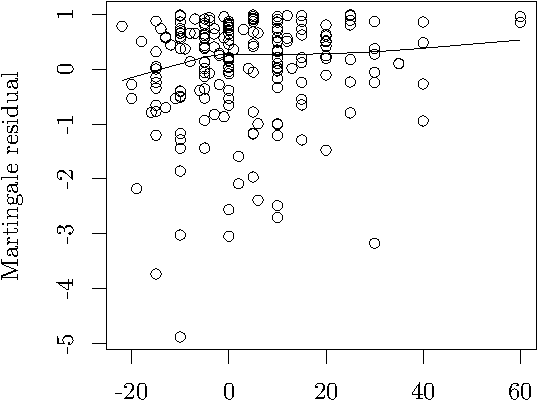
\includegraphics[width=\maxwidth]{figure/05-eda-func-form-size-1} 

}


\begin{kframe}\begin{alltt}
\hlkwd{scatter.smooth}\hlstd{(data}\hlopt{$}\hlstd{SizeCent,} \hlkwd{resid}\hlstd{(fit.cph.NoSize,} \hlkwc{type} \hlstd{=} \hlstr{"martingale"}\hlstd{),} \hlkwc{xlab} \hlstd{=} \hlstr{""}\hlstd{,} \hlkwc{ylab} \hlstd{=} \hlstr{"Martingale residual"}\hlstd{,} \hlkwc{ylim} \hlstd{=} \hlkwd{c}\hlstd{(}\hlopt{-}\hlnum{1}\hlstd{,} \hlnum{1}\hlstd{))}
\end{alltt}
\end{kframe}

{\centering 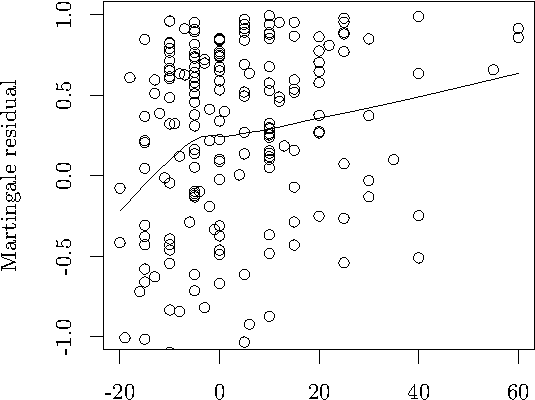
\includegraphics[width=\maxwidth]{figure/05-eda-func-form-size-2} 

}



\end{knitrout}
It looks like age has a minor nonlinear component, leading to a quadratic-like U shape.  The size relationship appears to have a knee, close to size == 0, around which the relationship is approximately linear.

Model age as:  $AgeCent + AgeCent^2$
Model size as: $SizeCent + SizeCent I(SizeCent > 0) \equiv SizeCent + SizeCent_+$

\begin{knitrout}
\definecolor{shadecolor}{rgb}{0.969, 0.969, 0.969}\color{fgcolor}\begin{kframe}
\begin{alltt}
\hlstd{data}\hlopt{$}\hlstd{SizeSmall} \hlkwb{=} \hlstd{data}\hlopt{$}\hlstd{SizeCent} \hlopt{*} \hlstd{(data}\hlopt{$}\hlstd{SizeCent} \hlopt{<} \hlnum{0}\hlstd{)}
\hlstd{data}\hlopt{$}\hlstd{AgeCent2} \hlkwb{=} \hlstd{data}\hlopt{$}\hlstd{AgeCent}\hlopt{^}\hlnum{2}
\end{alltt}
\end{kframe}
\end{knitrout}

\subsection{PH assumption: full model}
\begin{knitrout}
\definecolor{shadecolor}{rgb}{0.969, 0.969, 0.969}\color{fgcolor}\begin{kframe}
\begin{alltt}
\hlstd{fit.cph} \hlkwb{=} \hlkwd{coxph}\hlstd{(}\hlkwd{Surv}\hlstd{(Time, DSD)} \hlopt{~} \hlstd{SexM} \hlopt{+} \hlstd{AgeCent} \hlopt{+} \hlstd{AgeCent2} \hlopt{+} \hlstd{LocBody} \hlopt{+} \hlstd{SizeCent} \hlopt{+} \hlstd{SizeSmall} \hlopt{+} \hlstd{A2} \hlopt{+} \hlstd{A4,} \hlkwc{data} \hlstd{= data)}
\hlkwd{cox.zph}\hlstd{(fit.cph)}
\end{alltt}
\begin{verbatim}
##                 rho   chisq      p
## SexMTRUE     0.1520  4.2830 0.0385
## AgeCent     -0.0897  1.5736 0.2097
## AgeCent2     0.0392  0.2733 0.6012
## LocBodyTRUE -0.1287  2.7244 0.0988
## SizeCent     0.0088  0.0168 0.8970
## SizeSmall   -0.0592  0.6803 0.4095
## A2TRUE       0.0533  0.5483 0.4590
## A4TRUE      -0.0596  0.6487 0.4206
## GLOBAL           NA 14.0077 0.0816
\end{verbatim}
\begin{alltt}
\hlkwd{plot}\hlstd{(}\hlkwd{cox.zph}\hlstd{(fit.cph))}
\end{alltt}
\end{kframe}

{\centering 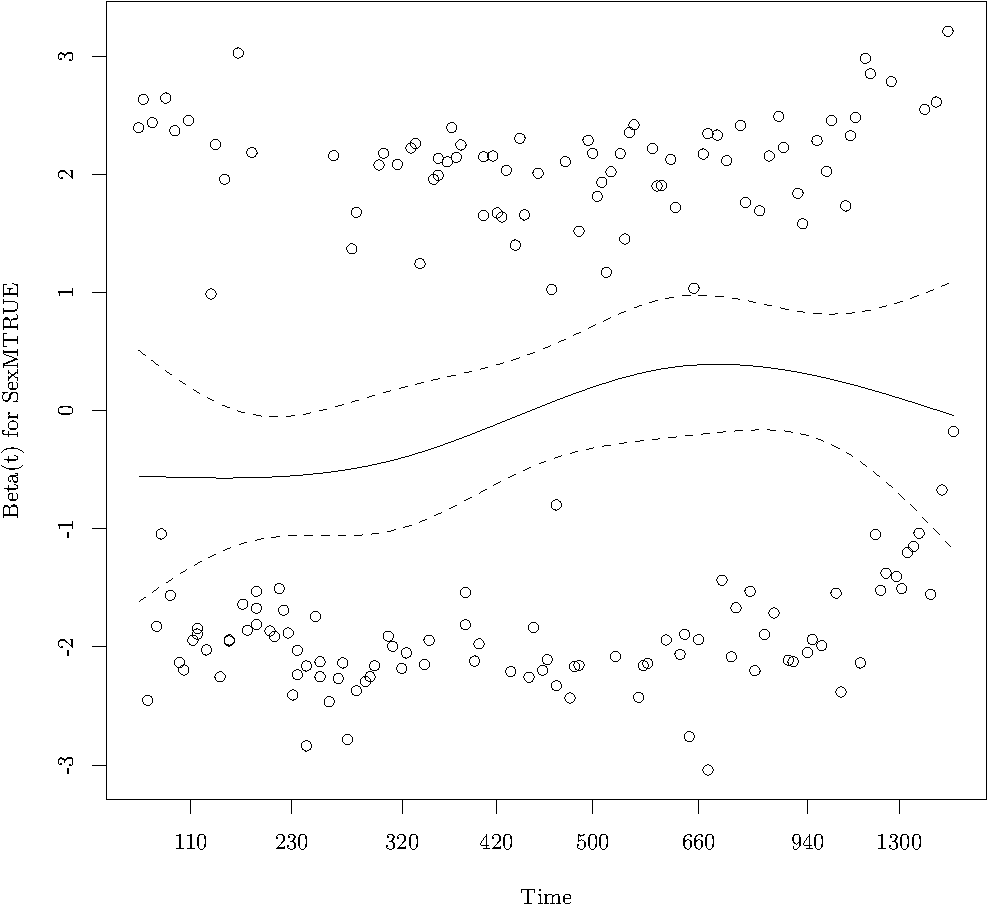
\includegraphics[width=\maxwidth]{figure/05-eda-ph-check-full-1} 

}




{\centering 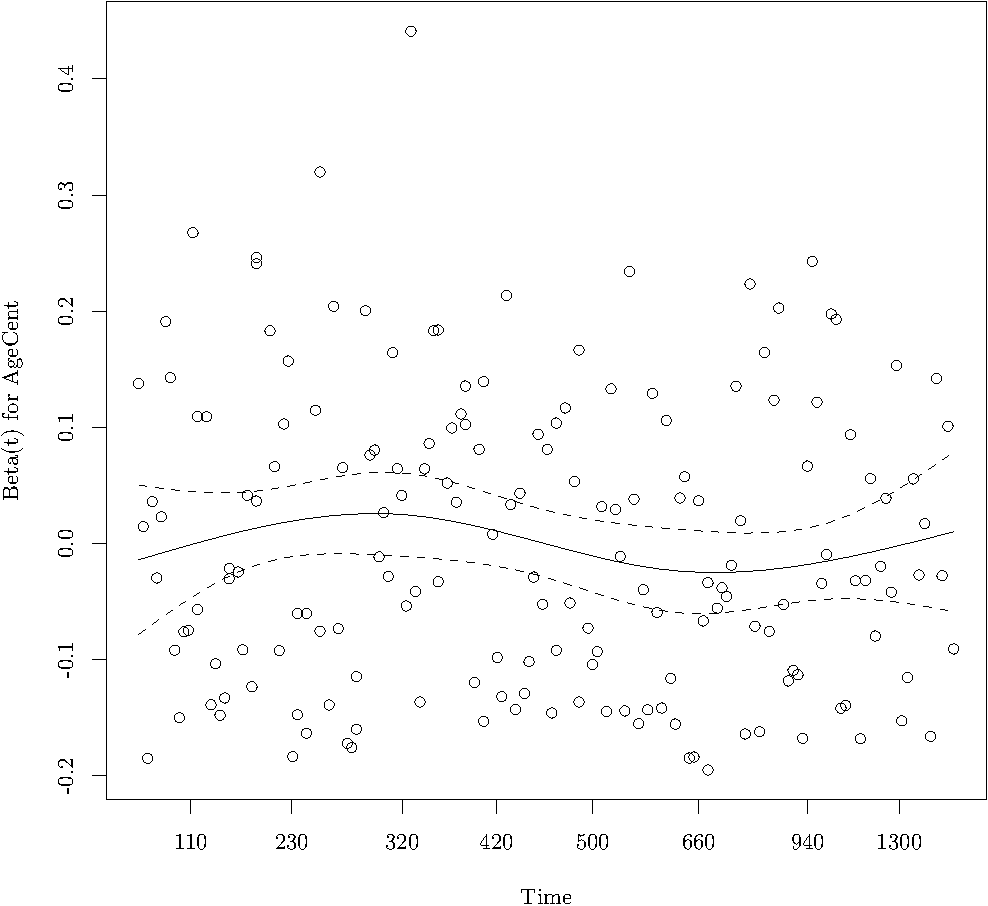
\includegraphics[width=\maxwidth]{figure/05-eda-ph-check-full-2} 

}




{\centering 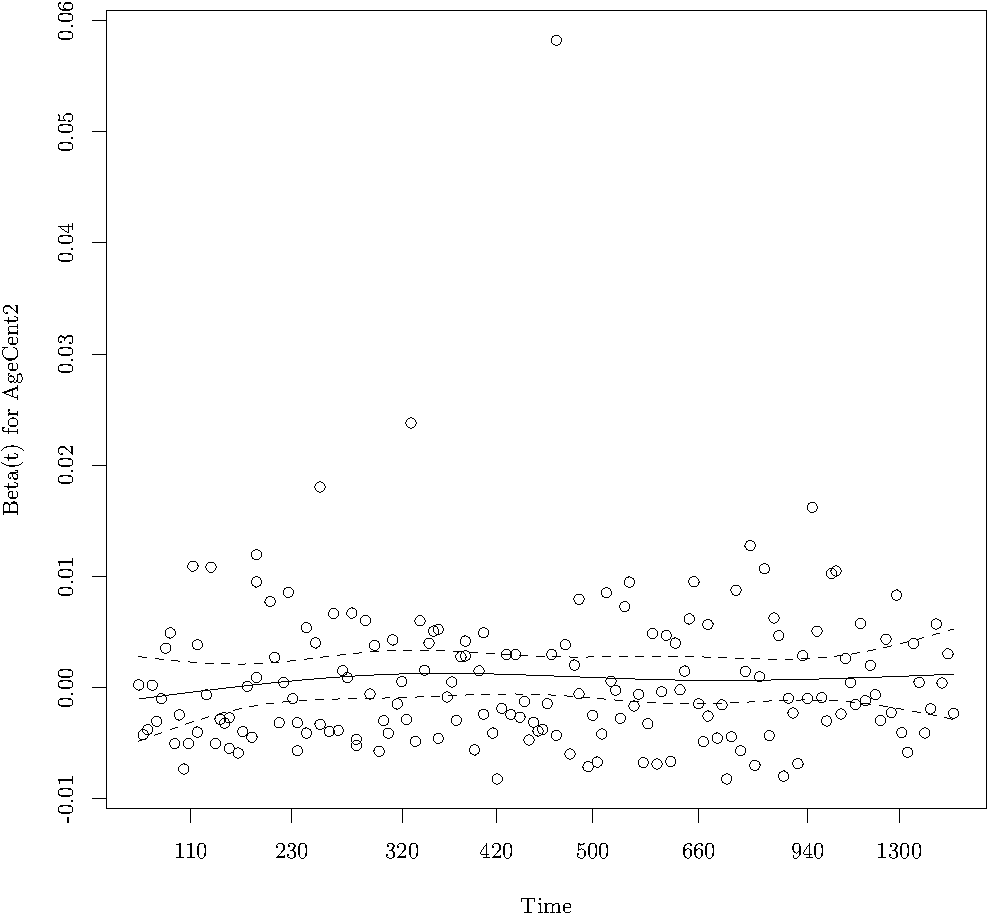
\includegraphics[width=\maxwidth]{figure/05-eda-ph-check-full-3} 

}




{\centering 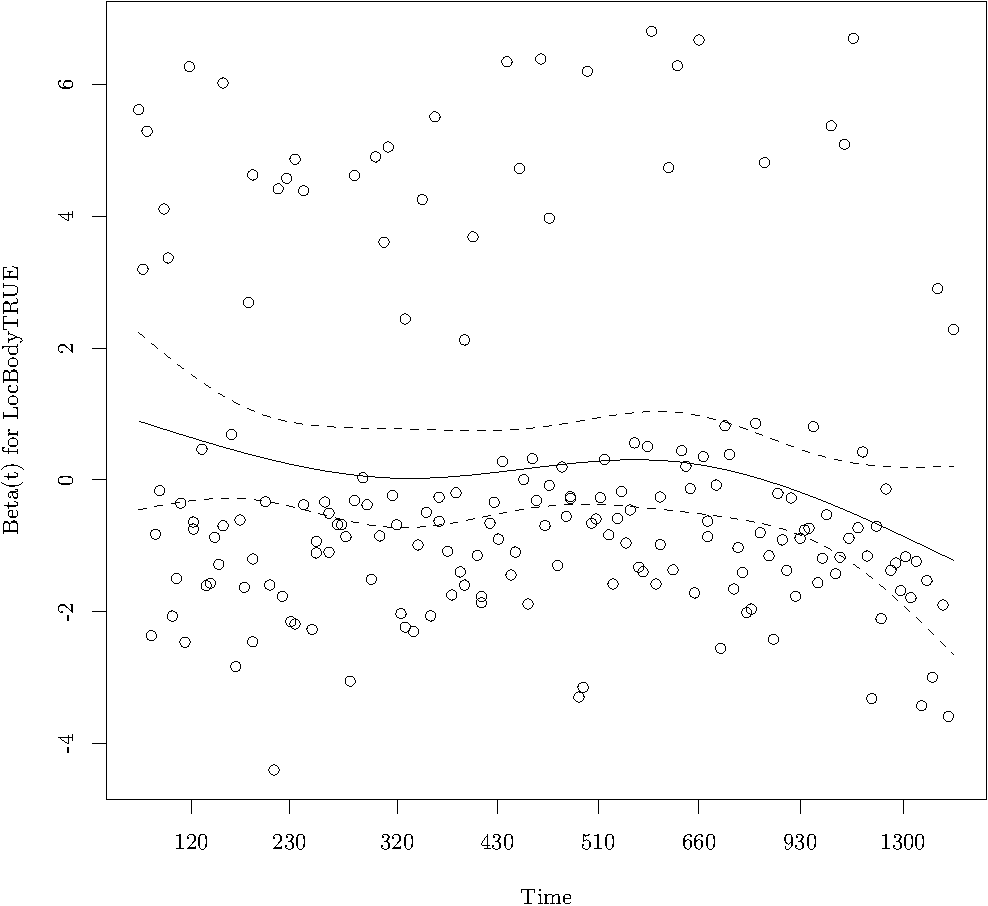
\includegraphics[width=\maxwidth]{figure/05-eda-ph-check-full-4} 

}




{\centering 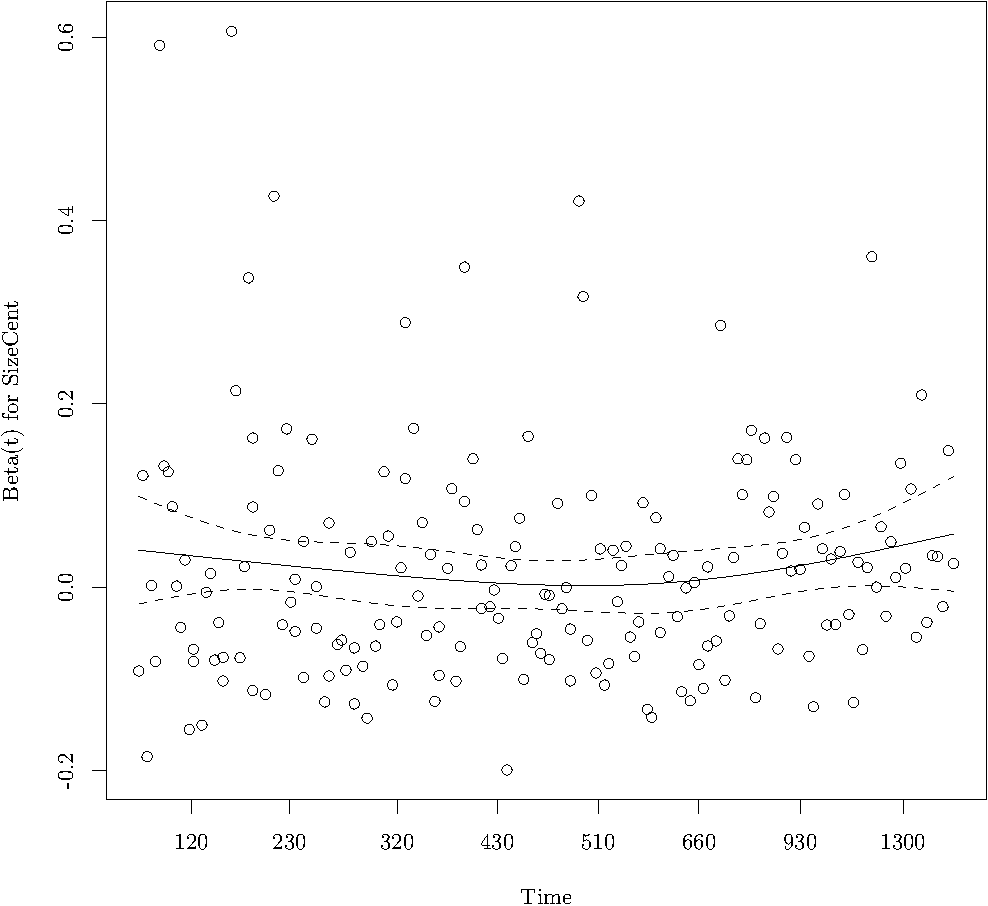
\includegraphics[width=\maxwidth]{figure/05-eda-ph-check-full-5} 

}




{\centering 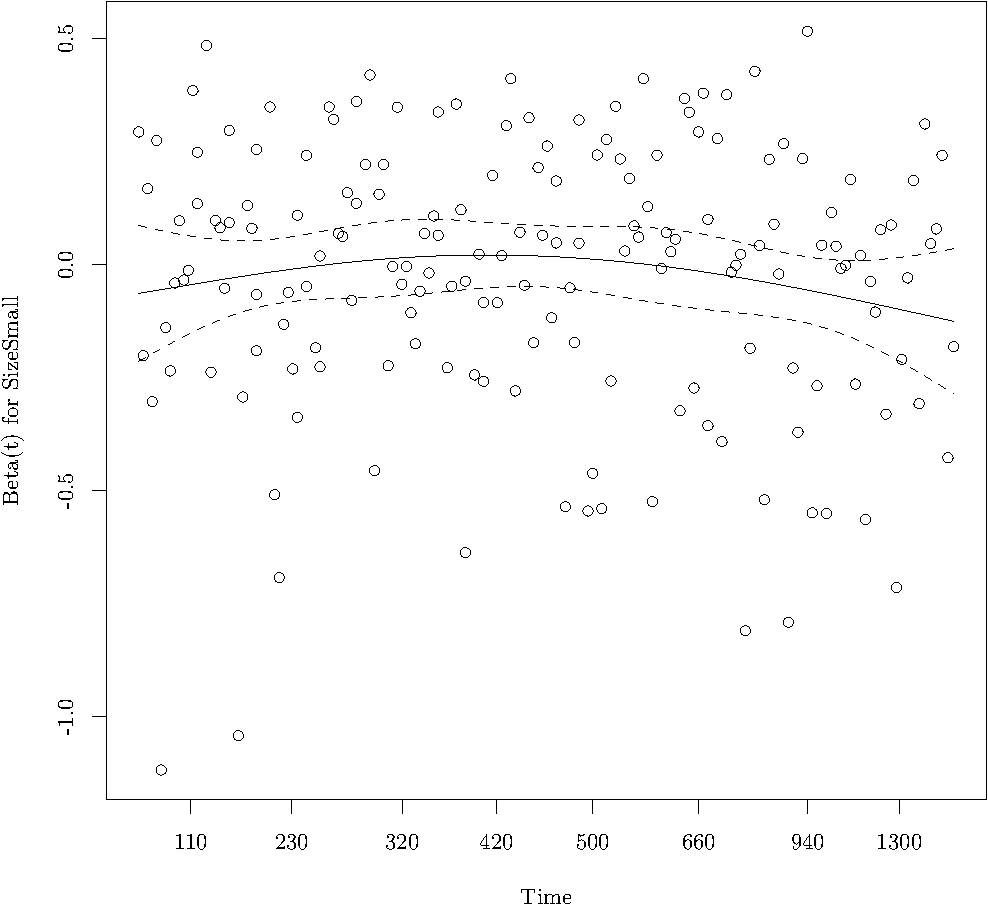
\includegraphics[width=\maxwidth]{figure/05-eda-ph-check-full-6} 

}




{\centering 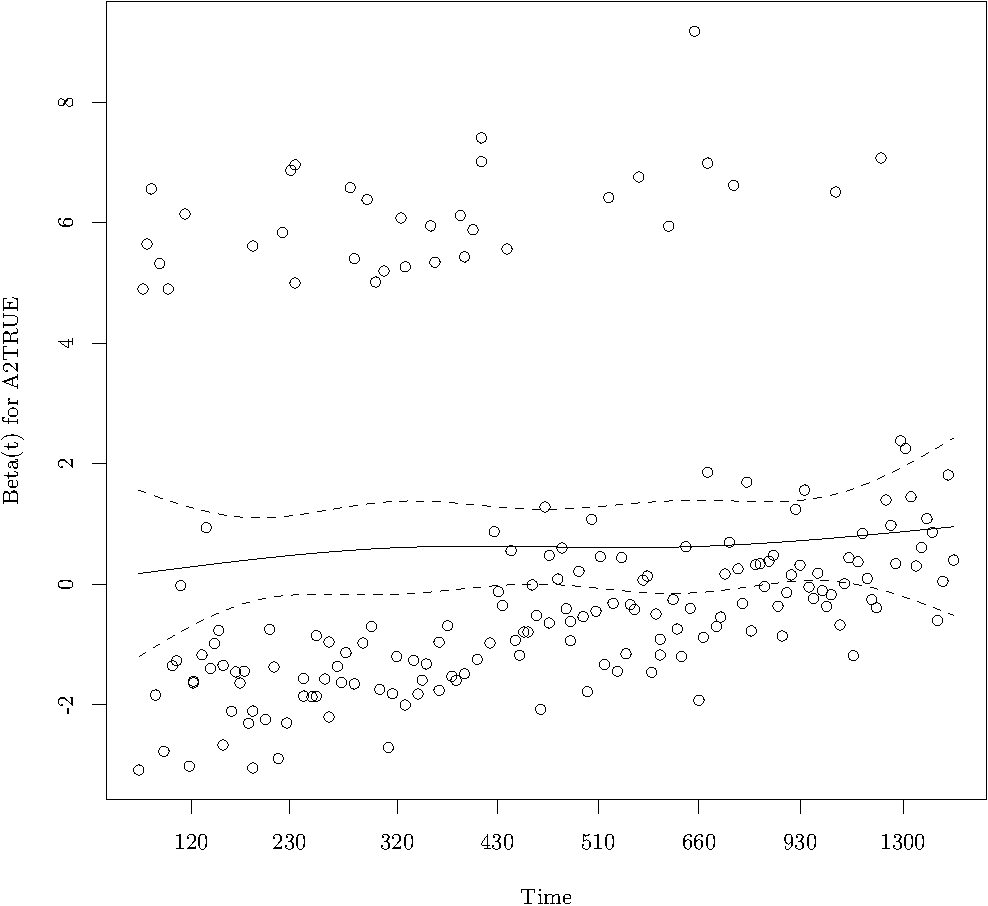
\includegraphics[width=\maxwidth]{figure/05-eda-ph-check-full-7} 

}




{\centering 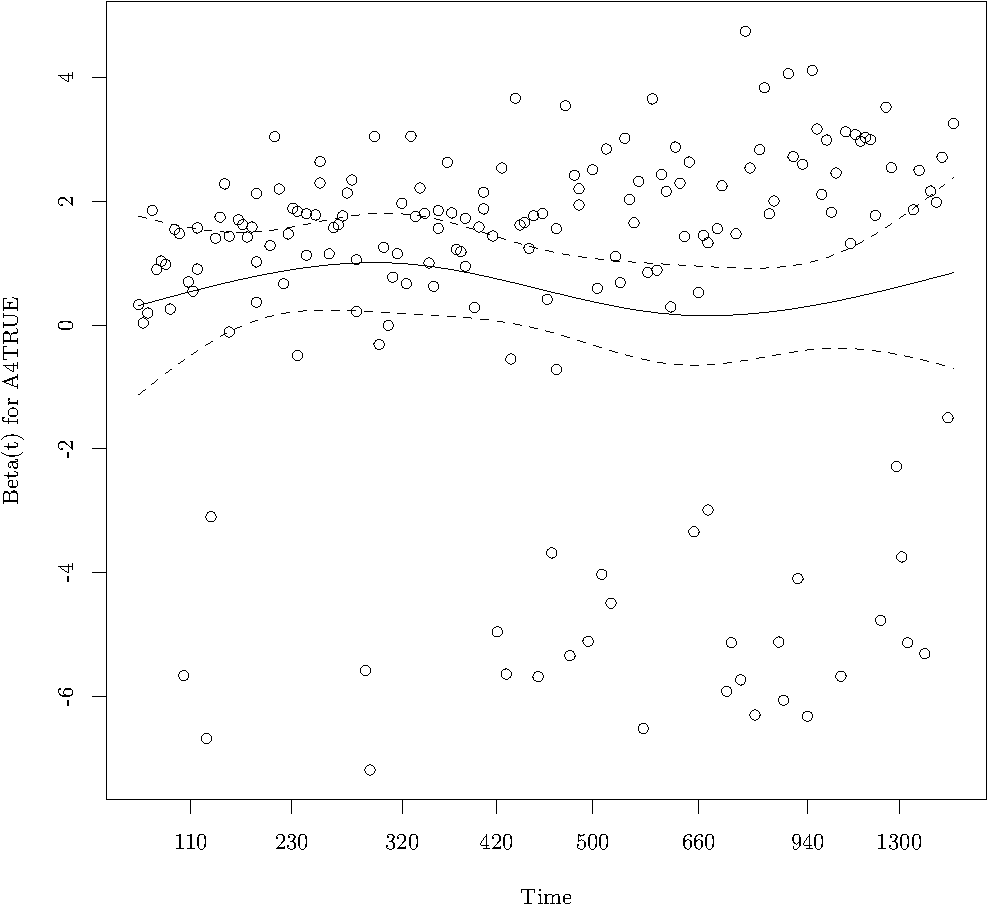
\includegraphics[width=\maxwidth]{figure/05-eda-ph-check-full-8} 

}



\end{knitrout}

\begin{knitrout}
\definecolor{shadecolor}{rgb}{0.969, 0.969, 0.969}\color{fgcolor}\begin{kframe}
\begin{alltt}
\hlstd{temp} \hlkwb{=} \hlkwa{function} \hlstd{(}\hlkwc{x}\hlstd{,} \hlkwc{resid} \hlstd{=} \hlnum{TRUE}\hlstd{,} \hlkwc{se} \hlstd{=} \hlnum{TRUE}\hlstd{,} \hlkwc{df} \hlstd{=} \hlnum{4}\hlstd{,} \hlkwc{nsmo} \hlstd{=} \hlnum{40}\hlstd{,} \hlkwc{var}\hlstd{,} \hlkwc{...}\hlstd{) \{}
    \hlstd{xx} \hlkwb{<-} \hlstd{x}\hlopt{$}\hlstd{x}
    \hlstd{yy} \hlkwb{<-} \hlstd{x}\hlopt{$}\hlstd{y}
    \hlstd{d} \hlkwb{<-} \hlkwd{nrow}\hlstd{(yy)}
    \hlstd{df} \hlkwb{<-} \hlkwd{max}\hlstd{(df)}
    \hlstd{nvar} \hlkwb{<-} \hlkwd{ncol}\hlstd{(yy)}
    \hlstd{pred.x} \hlkwb{<-} \hlkwd{seq}\hlstd{(}\hlkwc{from} \hlstd{=} \hlkwd{min}\hlstd{(xx),} \hlkwc{to} \hlstd{=} \hlkwd{max}\hlstd{(xx),} \hlkwc{length} \hlstd{= nsmo)}
    \hlstd{temp} \hlkwb{<-} \hlkwd{c}\hlstd{(pred.x, xx)}
    \hlstd{lmat} \hlkwb{<-} \hlkwd{ns}\hlstd{(temp,} \hlkwc{df} \hlstd{= df,} \hlkwc{intercept} \hlstd{=} \hlnum{TRUE}\hlstd{)}
    \hlstd{pmat} \hlkwb{<-} \hlstd{lmat[}\hlnum{1}\hlopt{:}\hlstd{nsmo, ]}
    \hlstd{xmat} \hlkwb{<-} \hlstd{lmat[}\hlopt{-}\hlstd{(}\hlnum{1}\hlopt{:}\hlstd{nsmo), ]}
    \hlstd{qmat} \hlkwb{<-} \hlkwd{qr}\hlstd{(xmat)}
    \hlkwa{if} \hlstd{(qmat}\hlopt{$}\hlstd{rank} \hlopt{<} \hlstd{df)}
        \hlkwd{stop}\hlstd{(}\hlstr{"Spline fit is singular, try a smaller degrees of freedom"}\hlstd{)}
    \hlkwa{if} \hlstd{(se) \{}
        \hlstd{bk} \hlkwb{<-} \hlkwd{backsolve}\hlstd{(qmat}\hlopt{$}\hlstd{qr[}\hlnum{1}\hlopt{:}\hlstd{df,} \hlnum{1}\hlopt{:}\hlstd{df],} \hlkwd{diag}\hlstd{(df))}
        \hlstd{xtx} \hlkwb{<-} \hlstd{bk} \hlopt \hlkwd{t}\hlstd{(bk)}
        \hlstd{seval} \hlkwb{<-} \hlstd{d} \hlopt{*} \hlstd{((pmat} \hlopt \hlstd{xtx)} \hlopt{*} \hlstd{pmat)} \hlopt \hlkwd{rep}\hlstd{(}\hlnum{1}\hlstd{, df)}
    \hlstd{\}}
    \hlstd{ylab} \hlkwb{<-} \hlkwd{paste}\hlstd{(}\hlstr{"Beta(t) for"}\hlstd{,} \hlkwd{dimnames}\hlstd{(yy)[[}\hlnum{2}\hlstd{]])}
    \hlkwa{if} \hlstd{(}\hlkwd{missing}\hlstd{(var))}
        \hlstd{var} \hlkwb{<-} \hlnum{1}\hlopt{:}\hlstd{nvar}
    \hlkwa{else} \hlstd{\{}
        \hlkwa{if} \hlstd{(}\hlkwd{is.character}\hlstd{(var))}
            \hlstd{var} \hlkwb{<-} \hlkwd{match}\hlstd{(var,} \hlkwd{dimnames}\hlstd{(yy)[[}\hlnum{2}\hlstd{]])}
        \hlkwa{if} \hlstd{(}\hlkwd{any}\hlstd{(}\hlkwd{is.na}\hlstd{(var))} \hlopt{||} \hlkwd{max}\hlstd{(var)} \hlopt{>} \hlstd{nvar} \hlopt{||} \hlkwd{min}\hlstd{(var)} \hlopt{<}
            \hlnum{1}\hlstd{)}
            \hlkwd{stop}\hlstd{(}\hlstr{"Invalid variable requested"}\hlstd{)}
    \hlstd{\}}
    \hlkwa{if} \hlstd{(x}\hlopt{$}\hlstd{transform} \hlopt{==} \hlstr{"log"}\hlstd{) \{}
        \hlstd{xx} \hlkwb{<-} \hlkwd{exp}\hlstd{(xx)}
        \hlstd{pred.x} \hlkwb{<-} \hlkwd{exp}\hlstd{(pred.x)}
    \hlstd{\}}
    \hlkwa{else if} \hlstd{(x}\hlopt{$}\hlstd{transform} \hlopt{!=} \hlstr{"identity"}\hlstd{) \{}
        \hlstd{xtime} \hlkwb{<-} \hlkwd{as.numeric}\hlstd{(}\hlkwd{dimnames}\hlstd{(yy)[[}\hlnum{1}\hlstd{]])}
        \hlstd{indx} \hlkwb{<-} \hlopt{!}\hlkwd{duplicated}\hlstd{(xx)}
        \hlstd{apr1} \hlkwb{<-} \hlkwd{approx}\hlstd{(xx[indx], xtime[indx],} \hlkwd{seq}\hlstd{(}\hlkwd{min}\hlstd{(xx),} \hlkwd{max}\hlstd{(xx),}
            \hlkwc{length} \hlstd{=} \hlnum{17}\hlstd{)[}\hlnum{2} \hlopt{*} \hlstd{(}\hlnum{1}\hlopt{:}\hlnum{8}\hlstd{)])}
        \hlstd{temp} \hlkwb{<-} \hlkwd{signif}\hlstd{(apr1}\hlopt{$}\hlstd{y,} \hlnum{2}\hlstd{)}
        \hlstd{apr2} \hlkwb{<-} \hlkwd{approx}\hlstd{(xtime[indx], xx[indx], temp)}
        \hlstd{xaxisval} \hlkwb{<-} \hlstd{apr2}\hlopt{$}\hlstd{y}
        \hlstd{xaxislab} \hlkwb{<-} \hlkwd{rep}\hlstd{(}\hlstr{""}\hlstd{,} \hlnum{8}\hlstd{)}
        \hlkwa{for} \hlstd{(i} \hlkwa{in} \hlnum{1}\hlopt{:}\hlnum{8}\hlstd{) xaxislab[i]} \hlkwb{<-} \hlkwd{format}\hlstd{(temp[i])}
    \hlstd{\}}
    \hlkwa{for} \hlstd{(i} \hlkwa{in} \hlstd{var) \{}
        \hlstd{y} \hlkwb{<-} \hlstd{yy[, i]}
        \hlstd{yhat} \hlkwb{<-} \hlstd{pmat} \hlopt \hlkwd{qr.coef}\hlstd{(qmat, y)}
        \hlkwa{if} \hlstd{(resid)}
            \hlstd{yr} \hlkwb{<-} \hlkwd{range}\hlstd{(yhat, y)}
        \hlkwa{else} \hlstd{yr} \hlkwb{<-} \hlkwd{range}\hlstd{(yhat)}
        \hlkwa{if} \hlstd{(se) \{}
            \hlstd{temp} \hlkwb{<-} \hlnum{2} \hlopt{*} \hlkwd{sqrt}\hlstd{(x}\hlopt{$}\hlstd{var[i, i]} \hlopt{*} \hlstd{seval)}
            \hlstd{yup} \hlkwb{<-} \hlstd{yhat} \hlopt{+} \hlstd{temp}
            \hlstd{ylow} \hlkwb{<-} \hlstd{yhat} \hlopt{-} \hlstd{temp}
            \hlstd{yr} \hlkwb{<-} \hlkwd{range}\hlstd{(yr, yup, ylow)}
        \hlstd{\}}
        \hlkwa{if} \hlstd{(x}\hlopt{$}\hlstd{transform} \hlopt{==} \hlstr{"identity"}\hlstd{)}
            \hlkwd{plot}\hlstd{(}\hlkwd{range}\hlstd{(xx), yr,} \hlkwc{type} \hlstd{=} \hlstr{"n"}\hlstd{, ...)}
        \hlkwa{else if} \hlstd{(x}\hlopt{$}\hlstd{transform} \hlopt{==} \hlstr{"log"}\hlstd{)}
            \hlkwd{plot}\hlstd{(}\hlkwd{range}\hlstd{(xx), yr,} \hlkwc{type} \hlstd{=} \hlstr{"n"}\hlstd{,} \hlkwc{log} \hlstd{=} \hlstr{"x"}\hlstd{, ...)}
        \hlkwa{else} \hlstd{\{}
            \hlkwd{plot}\hlstd{(}\hlkwd{range}\hlstd{(xx), yr,} \hlkwc{type} \hlstd{=} \hlstr{"n"}\hlstd{,} \hlkwc{axes} \hlstd{=} \hlnum{FALSE}\hlstd{, ...)}
            \hlkwd{axis}\hlstd{(}\hlnum{1}\hlstd{, xaxisval, xaxislab)}
            \hlkwd{axis}\hlstd{(}\hlnum{2}\hlstd{)}
            \hlkwd{box}\hlstd{()}
        \hlstd{\}}
        \hlkwa{if} \hlstd{(resid)}
            \hlkwd{points}\hlstd{(xx, y)}
        \hlkwd{lines}\hlstd{(pred.x, yhat)}
        \hlkwa{if} \hlstd{(se) \{}
            \hlkwd{lines}\hlstd{(pred.x, yup,} \hlkwc{lty} \hlstd{=} \hlnum{2}\hlstd{)}
            \hlkwd{lines}\hlstd{(pred.x, ylow,} \hlkwc{lty} \hlstd{=} \hlnum{2}\hlstd{)}
        \hlstd{\}}
    \hlstd{\}}
\hlstd{\}}

\hlkwd{temp}\hlstd{(}\hlkwd{cox.zph}\hlstd{(fit.cph),} \hlkwc{var} \hlstd{=} \hlnum{1}\hlstd{,} \hlkwc{ylab} \hlstd{=} \hlstr{"Scaled Schoenfeld residual for patient sex"}\hlstd{,} \hlkwc{xlab} \hlstd{=} \hlstr{"Time"}\hlstd{)}
\hlkwd{abline}\hlstd{(}\hlkwc{h} \hlstd{=} \hlnum{0}\hlstd{,} \hlkwc{lty} \hlstd{=} \hlstr{"dotted"}\hlstd{)}
\end{alltt}
\end{kframe}

{\centering 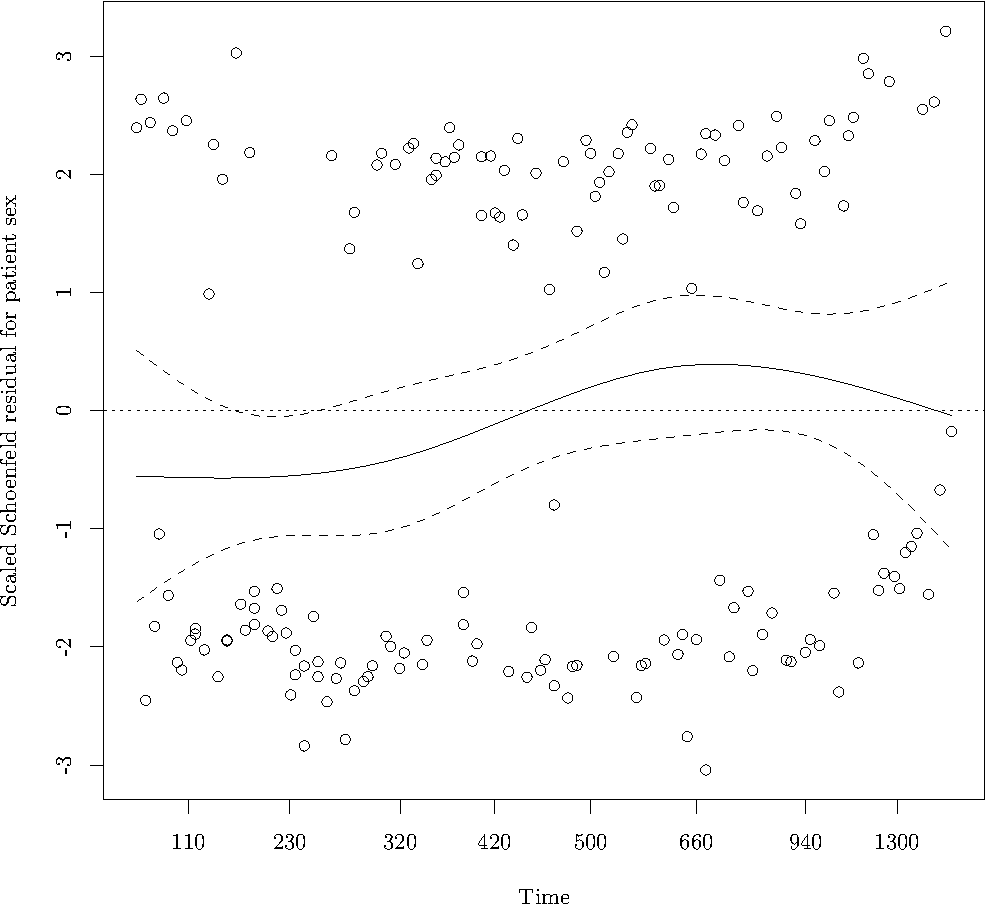
\includegraphics[width=\maxwidth]{figure/05-eda-ph-check-full-sexplot-1} 

}



\end{knitrout}


Looks like there's a violation of CPH with gender.  Not unexpected.  First check whether there is any evidence of gender interaction.
\begin{knitrout}
\definecolor{shadecolor}{rgb}{0.969, 0.969, 0.969}\color{fgcolor}\begin{kframe}
\begin{alltt}
\hlkwd{anova}\hlstd{(}\hlkwd{coxph}\hlstd{(}\hlkwd{Surv}\hlstd{(Time, DSD)} \hlopt{~} \hlstd{SexM}\hlopt{*}\hlstd{(AgeCent} \hlopt{+} \hlstd{AgeCent2} \hlopt{+} \hlstd{LocBody} \hlopt{+} \hlstd{SizeCent} \hlopt{+} \hlstd{SizeSmall} \hlopt{+} \hlstd{A2} \hlopt{+} \hlstd{A4),} \hlkwc{data} \hlstd{= data))}
\end{alltt}
\begin{verbatim}
## Analysis of Deviance Table
##  Cox model: response is Surv(Time, DSD)
## Terms added sequentially (first to last)
## 
##                loglik Chisq Df Pr(>|Chi|)
## NULL             -816                    
## SexM             -816  0.31  1     0.5770
## AgeCent          -816  0.00  1     0.9623
## AgeCent2         -815  0.78  1     0.3773
## LocBody          -813  3.45  1     0.0634
## SizeCent         -809  7.86  1     0.0050
## SizeSmall        -809  0.00  1     0.9983
## A2               -805  9.64  1     0.0019
## A4               -801  6.85  1     0.0088
## SexM:AgeCent     -800  1.65  1     0.1993
## SexM:AgeCent2    -800  0.00  1     0.9808
## SexM:LocBody     -800  0.10  1     0.7568
## SexM:SizeCent    -800  0.65  1     0.4218
## SexM:SizeSmall   -800  0.01  1     0.9108
## SexM:A2          -800  0.00  1     0.9960
## SexM:A4          -800  0.03  1     0.8537
\end{verbatim}
\end{kframe}
\end{knitrout}
Nope, good.  We're not interested in gender effects so just stratify.

\begin{knitrout}
\definecolor{shadecolor}{rgb}{0.969, 0.969, 0.969}\color{fgcolor}\begin{kframe}
\begin{alltt}
\hlstd{fit.cph} \hlkwb{=} \hlkwd{coxph}\hlstd{(}\hlkwd{Surv}\hlstd{(Time, DSD)} \hlopt{~} \hlkwd{strata}\hlstd{(SexM)} \hlopt{+} \hlstd{AgeCent} \hlopt{+} \hlstd{AgeCent2} \hlopt{+} \hlstd{LocBody} \hlopt{+} \hlstd{SizeCent} \hlopt{+} \hlstd{SizeSmall} \hlopt{+} \hlstd{A2} \hlopt{+} \hlstd{A4,} \hlkwc{data} \hlstd{= data)}
\hlkwd{cox.zph}\hlstd{(fit.cph)}
\end{alltt}
\begin{verbatim}
##                  rho  chisq     p
## AgeCent     -0.09066 1.6632 0.197
## AgeCent2     0.03371 0.2006 0.654
## LocBodyTRUE -0.10840 1.8729 0.171
## SizeCent    -0.00856 0.0157 0.900
## SizeSmall   -0.04531 0.3927 0.531
## A2TRUE       0.05681 0.6145 0.433
## A4TRUE      -0.06539 0.7755 0.379
## GLOBAL            NA 8.3356 0.304
\end{verbatim}
\begin{alltt}
\hlkwd{plot}\hlstd{(}\hlkwd{cox.zph}\hlstd{(fit.cph))}
\end{alltt}
\end{kframe}

{\centering 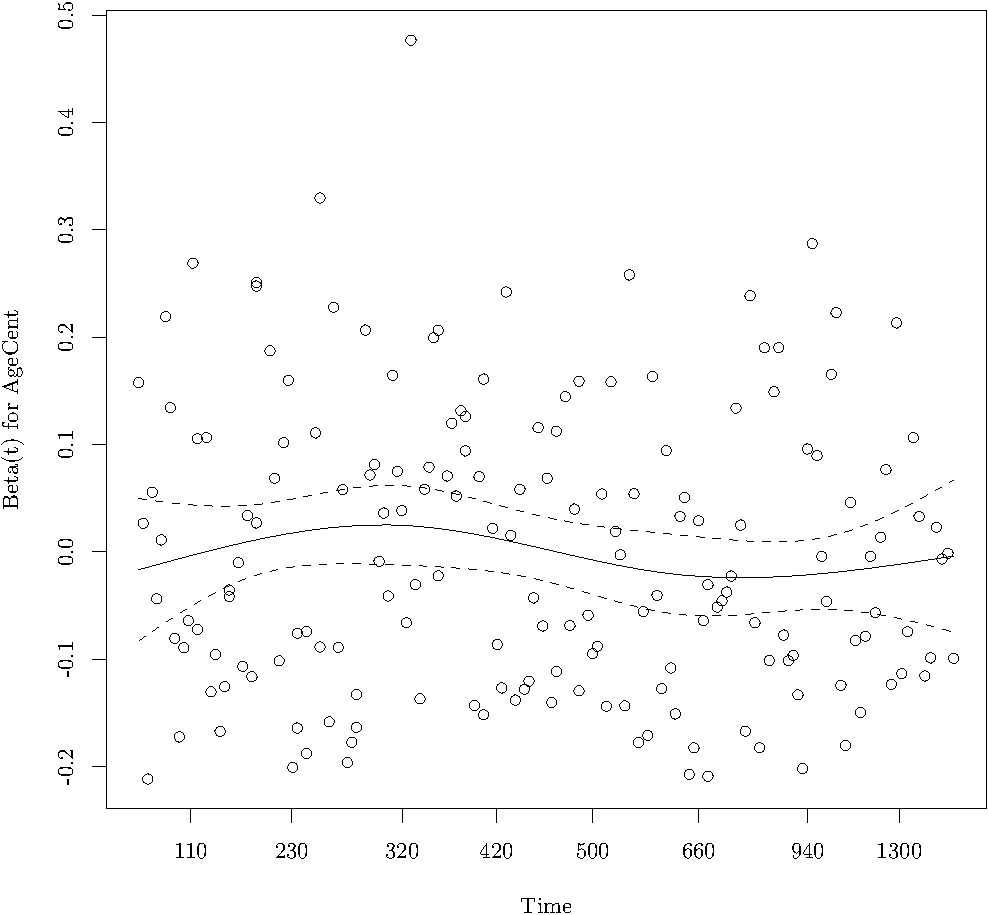
\includegraphics[width=\maxwidth]{figure/05-eda-ph-check-full-3-1} 

}




{\centering 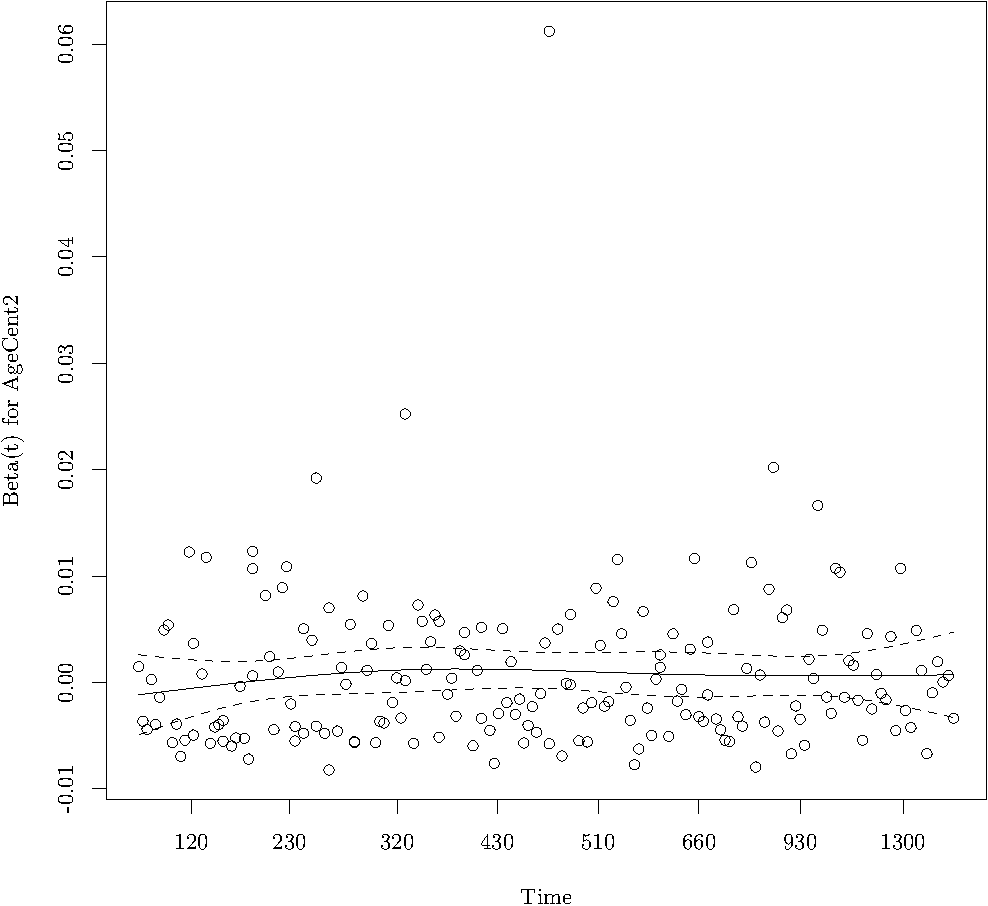
\includegraphics[width=\maxwidth]{figure/05-eda-ph-check-full-3-2} 

}




{\centering 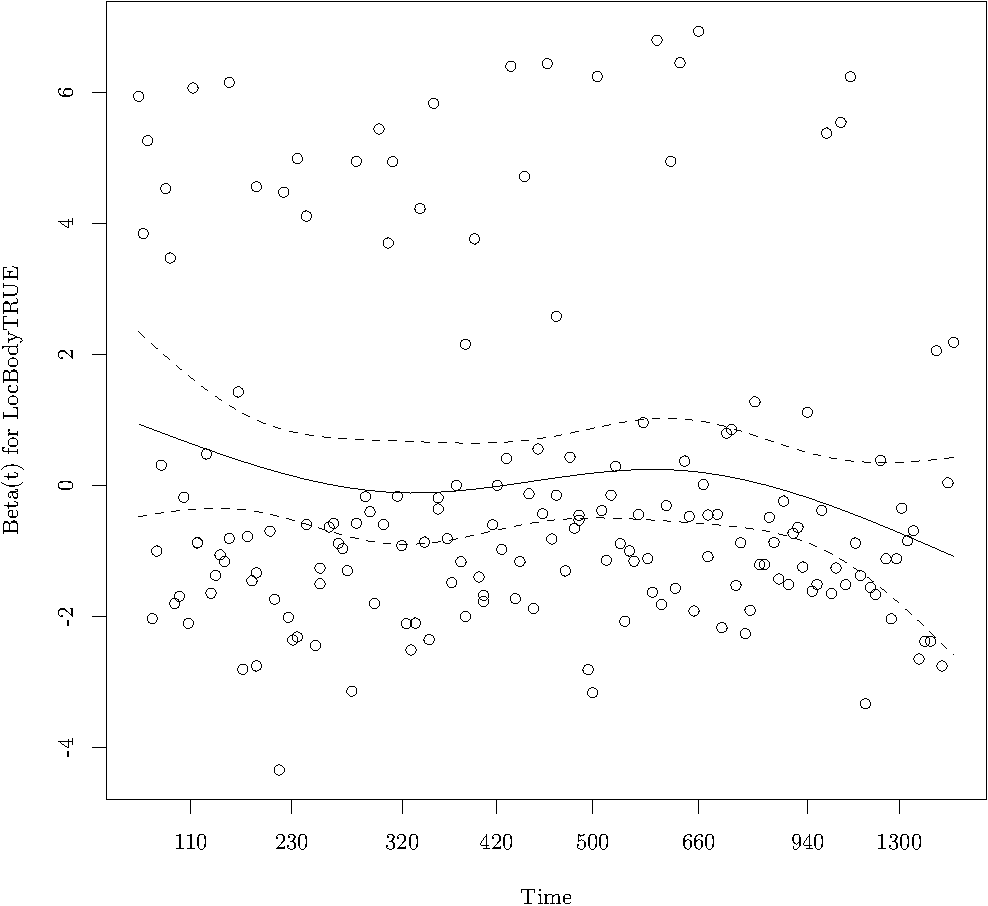
\includegraphics[width=\maxwidth]{figure/05-eda-ph-check-full-3-3} 

}




{\centering 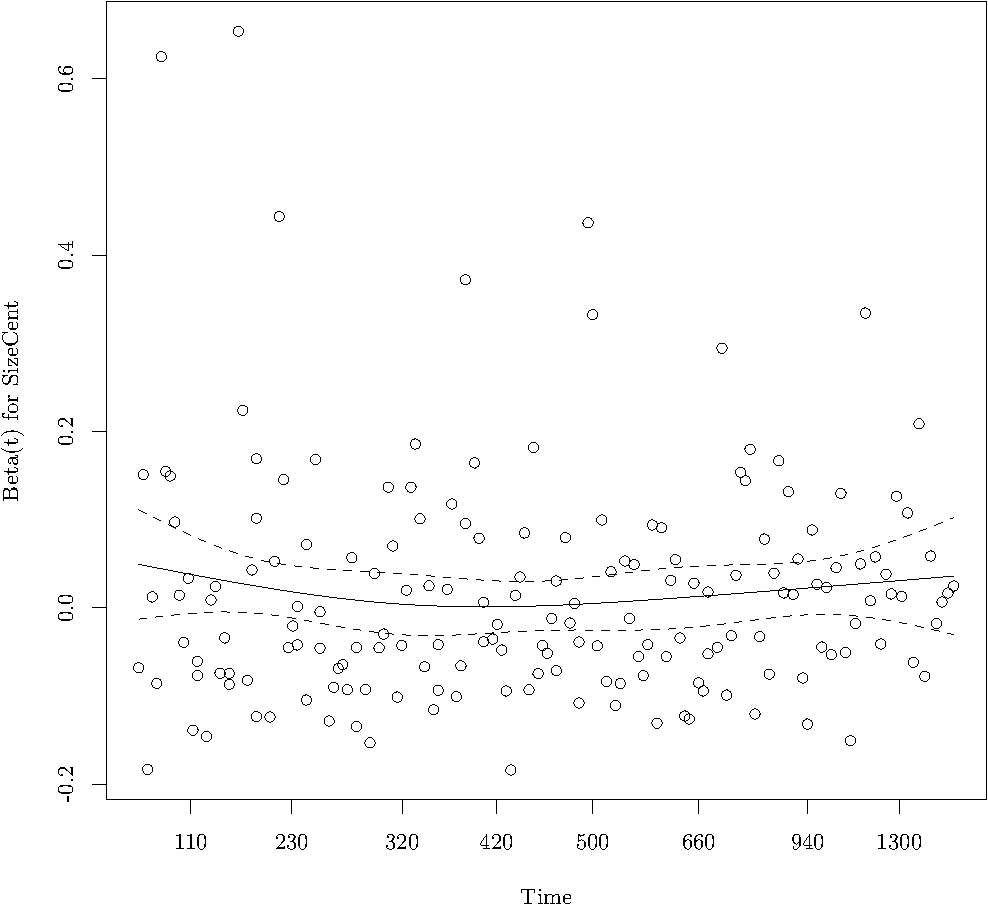
\includegraphics[width=\maxwidth]{figure/05-eda-ph-check-full-3-4} 

}




{\centering 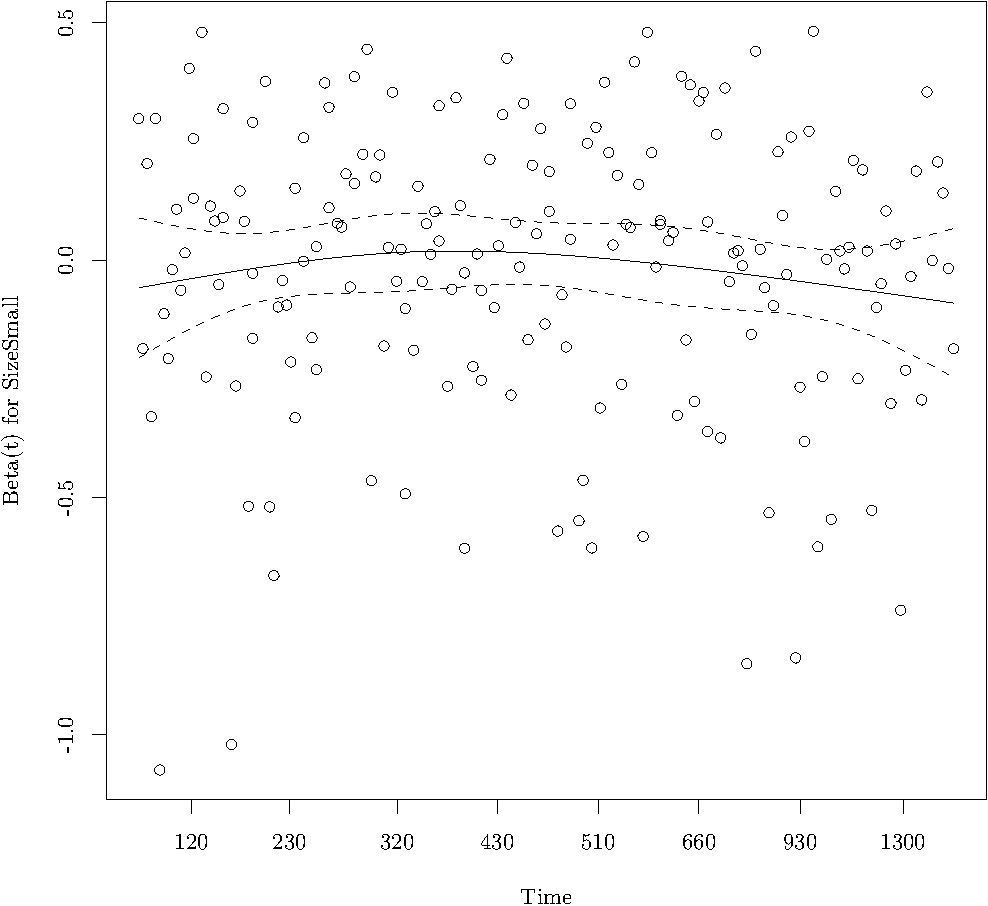
\includegraphics[width=\maxwidth]{figure/05-eda-ph-check-full-3-5} 

}




{\centering 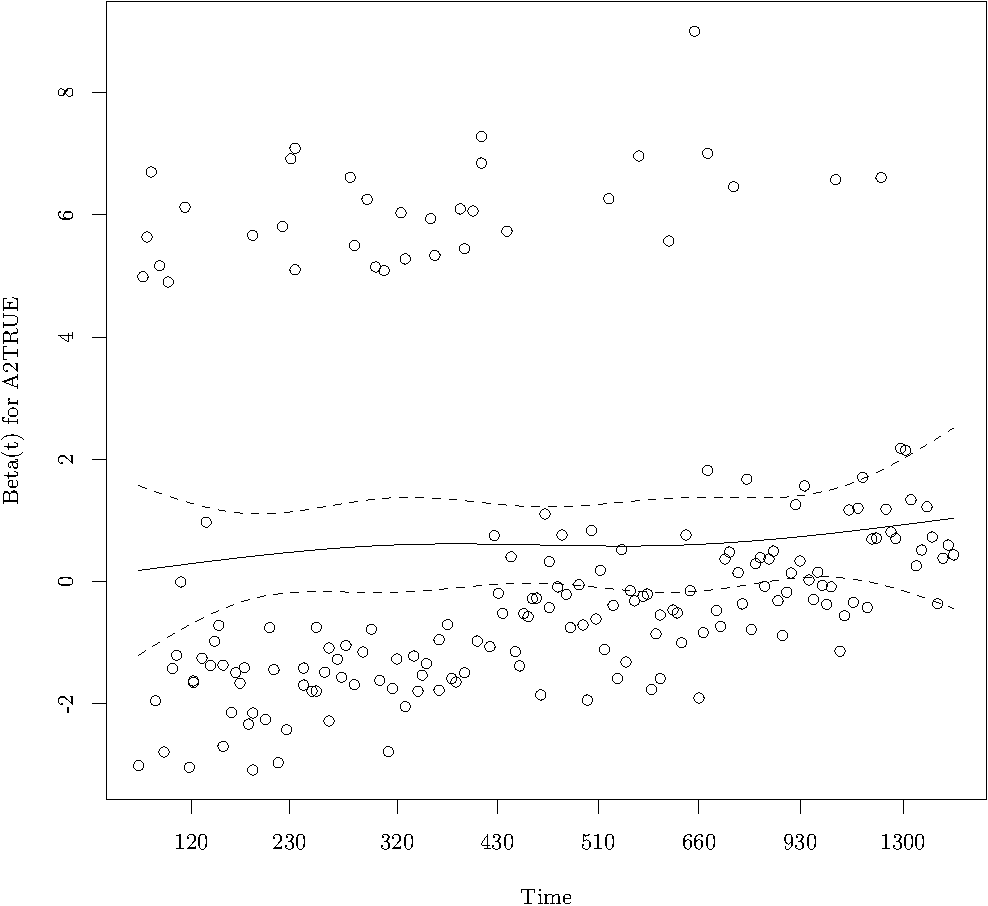
\includegraphics[width=\maxwidth]{figure/05-eda-ph-check-full-3-6} 

}




{\centering 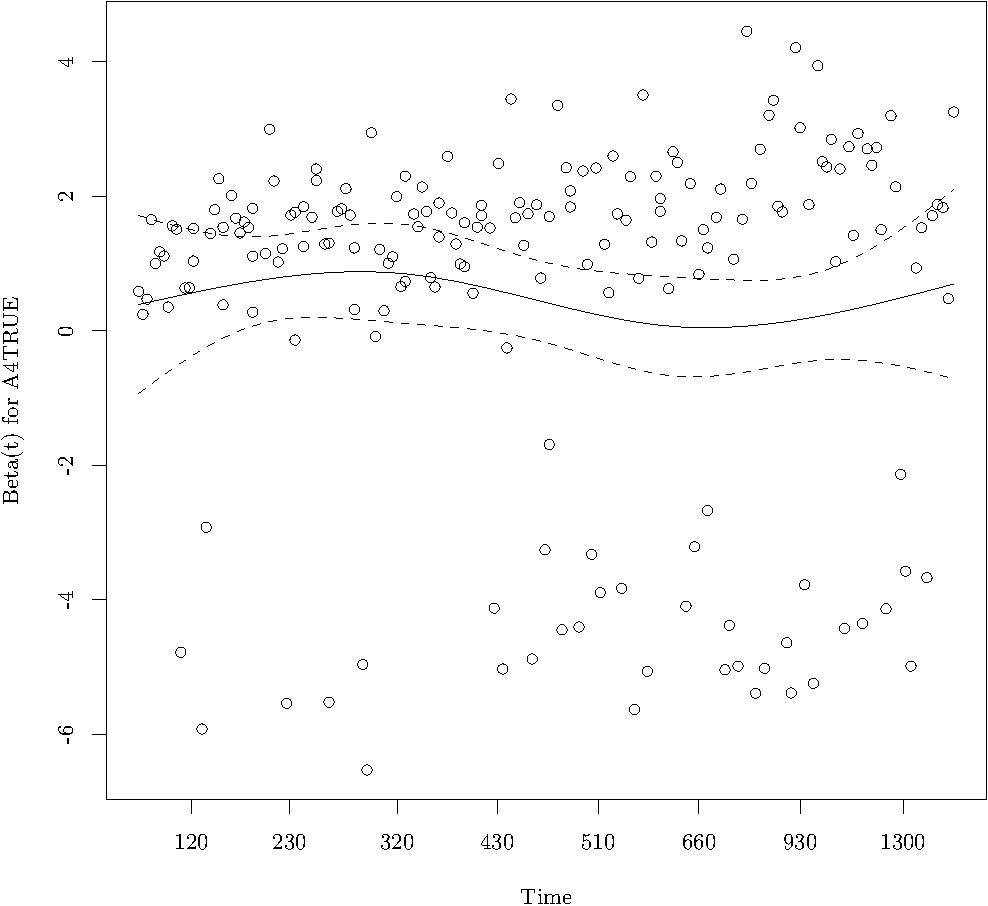
\includegraphics[width=\maxwidth]{figure/05-eda-ph-check-full-3-7} 

}



\end{knitrout}

Looks good.  Slight snifter with age but I'm not particularly concerned.
Split into age groups and do KM plots to verify.
\begin{knitrout}
\definecolor{shadecolor}{rgb}{0.969, 0.969, 0.969}\color{fgcolor}\begin{kframe}
\begin{alltt}
\hlstd{temp.age} \hlkwb{=} \hlkwd{cut}\hlstd{(data}\hlopt{$}\hlstd{AgeCent,} \hlnum{4}\hlstd{)}
\hlstd{temp} \hlkwb{=} \hlkwd{survfit}\hlstd{(}\hlkwd{Surv}\hlstd{(Time, DSD)} \hlopt{~} \hlstd{temp.age, data)}
\hlkwd{ggplot}\hlstd{(}\hlkwd{data.frame}\hlstd{(}\hlkwc{surv} \hlstd{= temp}\hlopt{$}\hlstd{surv,} \hlkwc{time} \hlstd{= temp}\hlopt{$}\hlstd{time,} \hlkwc{age} \hlstd{=} \hlkwd{rep}\hlstd{(}\hlkwd{names}\hlstd{(temp}\hlopt{$}\hlstd{strata), temp}\hlopt{$}\hlstd{strata)),} \hlkwd{aes}\hlstd{(}\hlkwc{y} \hlstd{=} \hlkwd{log}\hlstd{(}\hlopt{-}\hlkwd{log}\hlstd{(surv)),} \hlkwc{x} \hlstd{=} \hlkwd{log}\hlstd{(time),} \hlkwc{col} \hlstd{= age))} \hlopt{+} \hlkwd{geom_line}\hlstd{()}
\end{alltt}
\end{kframe}

{\centering 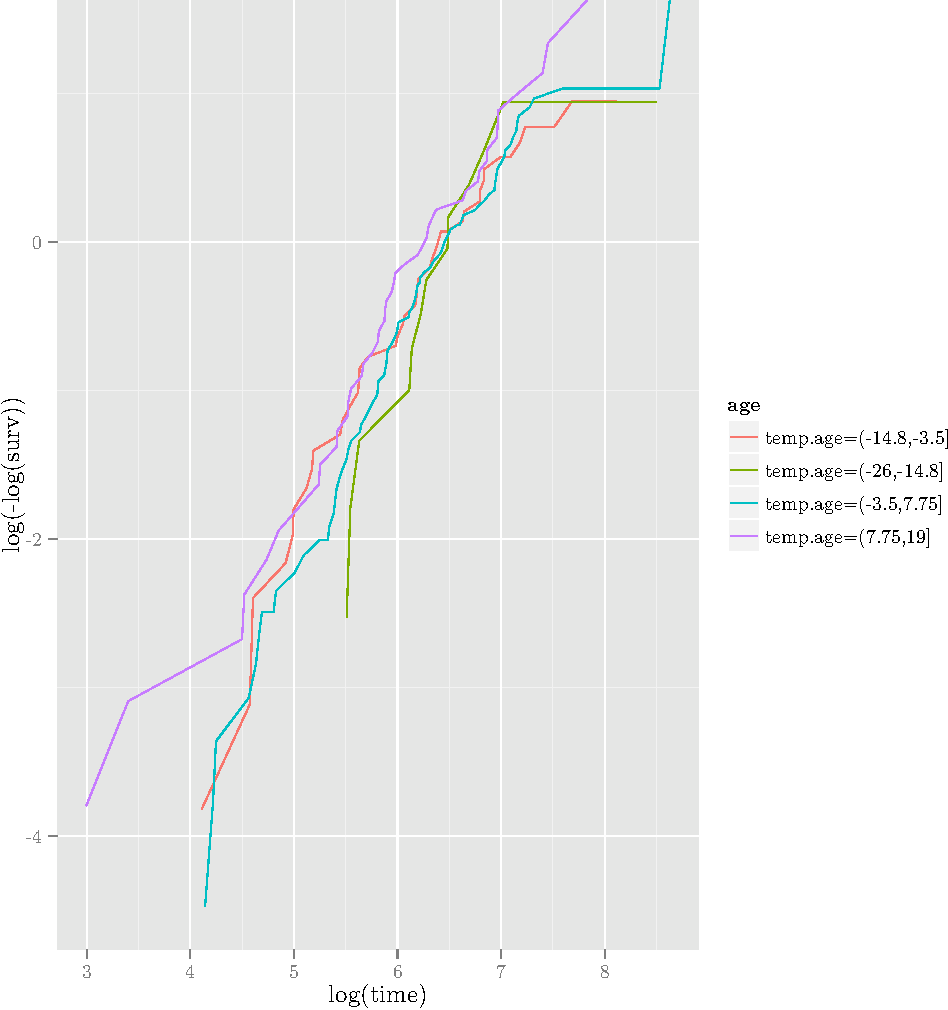
\includegraphics[width=\maxwidth]{figure/05-eda-ph-check-full-age-1} 

}



\end{knitrout}
Not perfect but it'll do.


\subsection{Outliers: full model}
Look at deviance residuals, both marginally and stratified by major subgroups.
\begin{knitrout}
\definecolor{shadecolor}{rgb}{0.969, 0.969, 0.969}\color{fgcolor}\begin{kframe}
\begin{alltt}
\hlkwd{plot}\hlstd{(}\hlkwd{resid}\hlstd{(fit.cph,} \hlkwc{type} \hlstd{=} \hlstr{"deviance"}\hlstd{))}
\hlkwd{abline}\hlstd{(}\hlkwc{h} \hlstd{=} \hlkwd{c}\hlstd{(}\hlopt{-}\hlnum{2.5}\hlstd{,} \hlnum{2.5}\hlstd{))}
\end{alltt}
\end{kframe}

{\centering 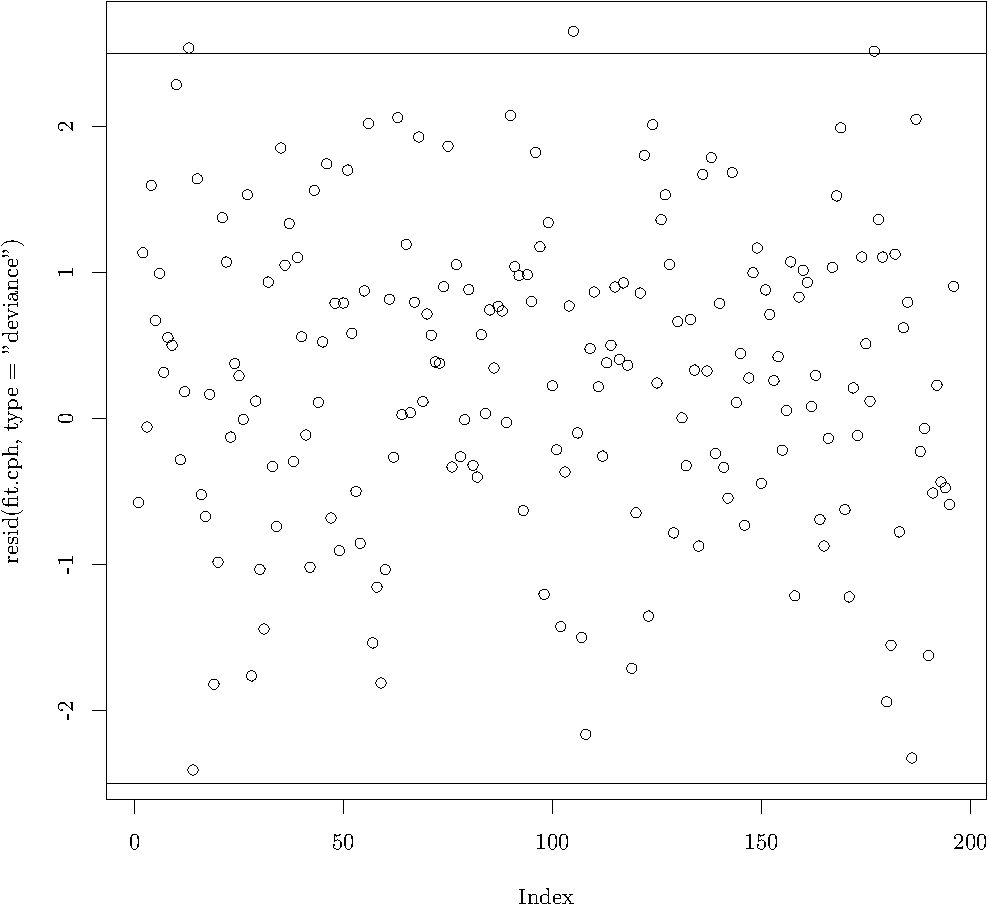
\includegraphics[width=\maxwidth]{figure/05-eda-outliers-full-1} 

}


\begin{kframe}\begin{alltt}
\hlstd{temp.ord} \hlkwb{=} \hlkwd{order}\hlstd{(data}\hlopt{$}\hlstd{SexM, data}\hlopt{$}\hlstd{A2, data}\hlopt{$}\hlstd{A4)}
\hlstd{temp.resid} \hlkwb{=} \hlkwd{resid}\hlstd{(fit.cph,} \hlkwc{type} \hlstd{=} \hlstr{"deviance"}\hlstd{)[temp.ord]}
\hlstd{temp.col} \hlkwb{=} \hlstd{(}\hlnum{4}\hlopt{*}\hlstd{data}\hlopt{$}\hlstd{SexM} \hlopt{+} \hlnum{2}\hlopt{*}\hlstd{data}\hlopt{$}\hlstd{A2} \hlopt{+} \hlstd{data}\hlopt{$}\hlstd{A4} \hlopt{+} \hlnum{1}\hlstd{)[temp.ord]}
\hlkwd{plot}\hlstd{(temp.resid,} \hlkwc{col} \hlstd{= temp.col,} \hlkwc{pch} \hlstd{=} \hlnum{16}\hlstd{)}
\hlkwd{abline}\hlstd{(}\hlkwc{h} \hlstd{=} \hlkwd{c}\hlstd{(}\hlopt{-}\hlnum{2.5}\hlstd{,} \hlnum{2.5}\hlstd{))}
\end{alltt}
\end{kframe}

{\centering 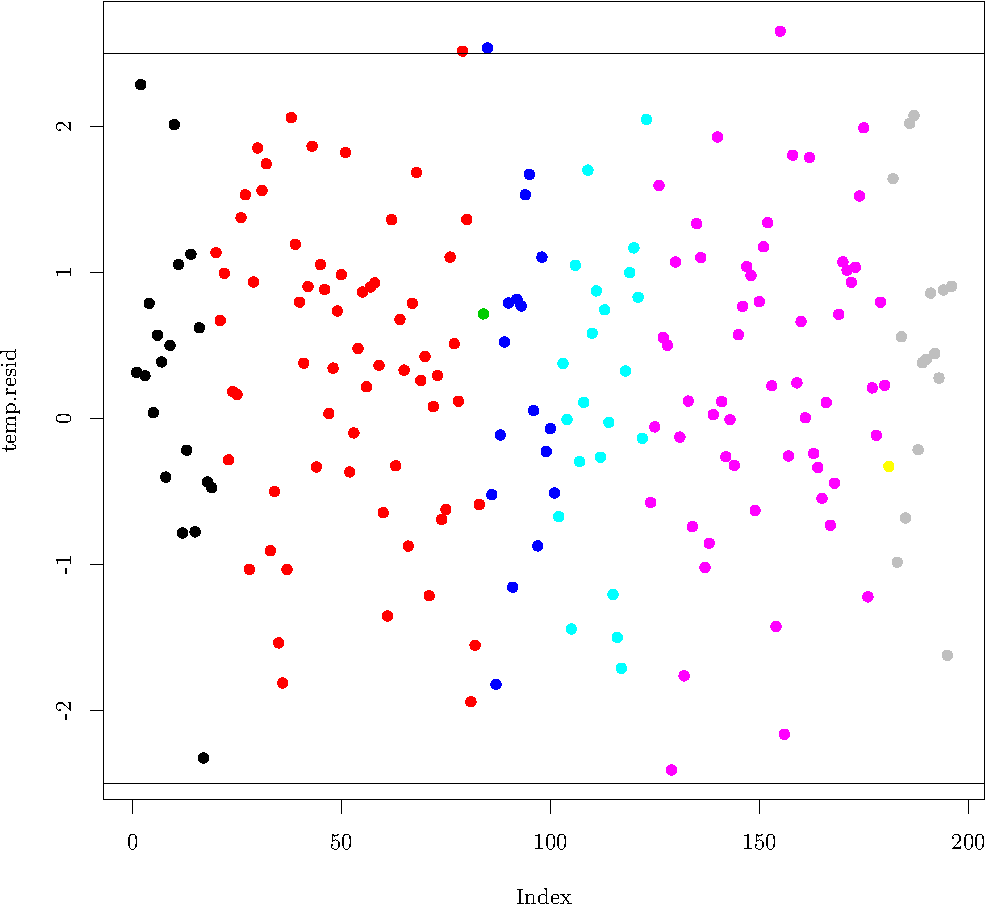
\includegraphics[width=\maxwidth]{figure/05-eda-outliers-full-2} 

}


\begin{kframe}\begin{alltt}
\hlkwd{boxplot}\hlstd{(}\hlkwd{resid}\hlstd{(fit.cph,} \hlkwc{type} \hlstd{=} \hlstr{"deviance"}\hlstd{)} \hlopt{~} \hlstd{data}\hlopt{$}\hlstd{SexM} \hlopt{+} \hlstd{data}\hlopt{$}\hlstd{A2} \hlopt{+} \hlstd{data}\hlopt{$}\hlstd{A4,} \hlkwc{varwidth} \hlstd{=} \hlnum{TRUE}\hlstd{)}
\hlkwd{abline}\hlstd{(}\hlkwc{h} \hlstd{=} \hlnum{0}\hlstd{)}
\end{alltt}
\end{kframe}

{\centering 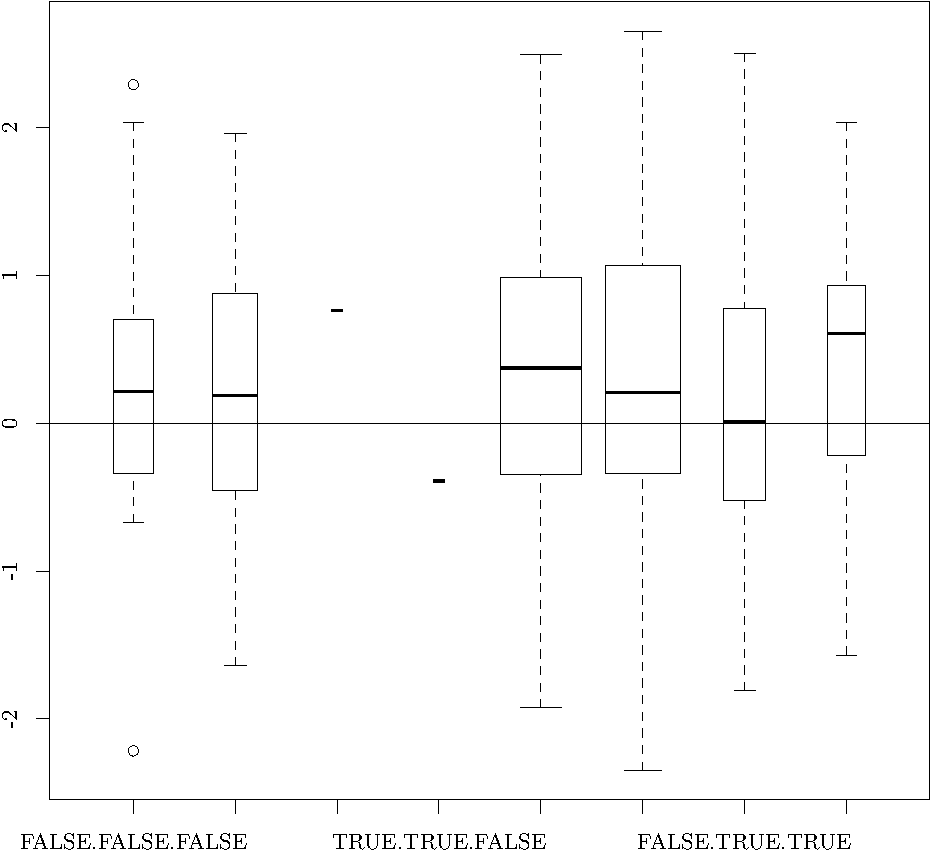
\includegraphics[width=\maxwidth]{figure/05-eda-outliers-full-3} 

}


\begin{kframe}\begin{alltt}
\hlkwd{boxplot}\hlstd{(}\hlkwd{resid}\hlstd{(fit.cph,} \hlkwc{type} \hlstd{=} \hlstr{"martingale"}\hlstd{)} \hlopt{~} \hlstd{data}\hlopt{$}\hlstd{SexM} \hlopt{+} \hlstd{data}\hlopt{$}\hlstd{A2} \hlopt{+} \hlstd{data}\hlopt{$}\hlstd{A4,} \hlkwc{varwidth} \hlstd{=} \hlnum{TRUE}\hlstd{)}
\hlkwd{abline}\hlstd{(}\hlkwc{h} \hlstd{=} \hlnum{0}\hlstd{)}
\end{alltt}
\end{kframe}

{\centering 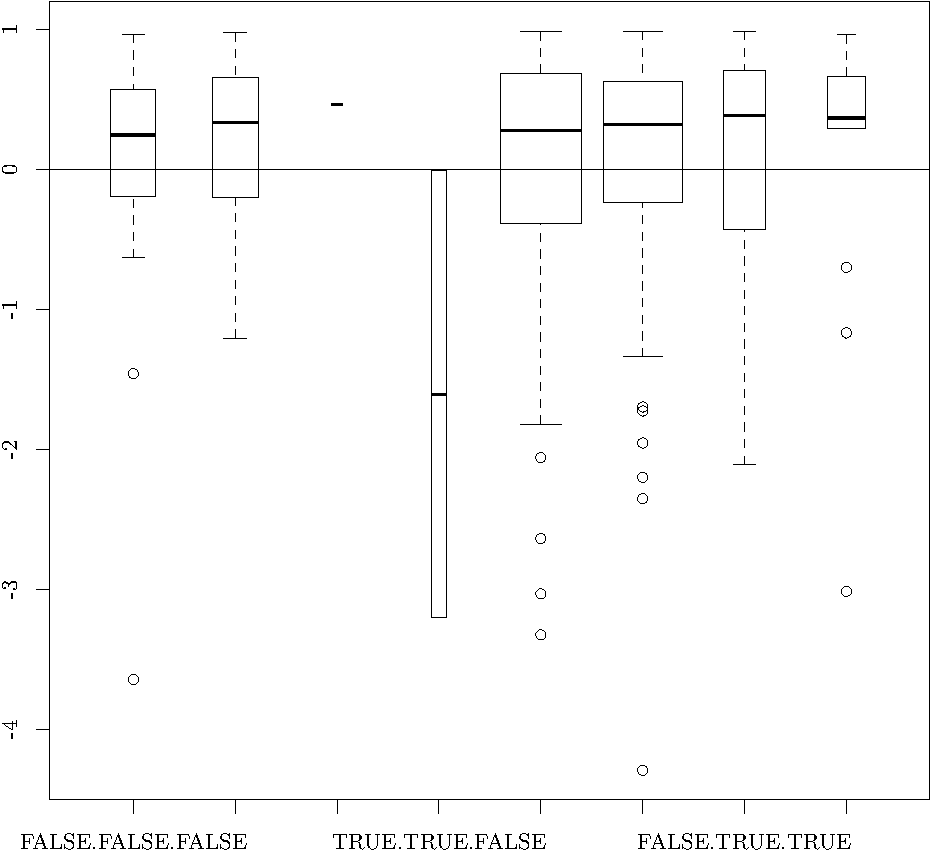
\includegraphics[width=\maxwidth]{figure/05-eda-outliers-full-4} 

}



\end{knitrout}

Use DFBETAS to examine influence.
\begin{knitrout}
\definecolor{shadecolor}{rgb}{0.969, 0.969, 0.969}\color{fgcolor}\begin{kframe}
\begin{alltt}
\hlstd{temp} \hlkwb{=} \hlkwd{resid}\hlstd{(fit.cph,} \hlkwc{type} \hlstd{=} \hlstr{"dfbetas"}\hlstd{)}
\hlkwd{colnames}\hlstd{(temp)} \hlkwb{=} \hlkwd{names}\hlstd{(fit.cph}\hlopt{$}\hlstd{coefficients)}
\hlstd{temp} \hlkwb{=} \hlkwd{melt}\hlstd{(temp)}
\hlkwd{colnames}\hlstd{(temp)} \hlkwb{=} \hlkwd{c}\hlstd{(}\hlstr{"Patient"}\hlstd{,} \hlstr{"Coefficient"}\hlstd{,} \hlstr{"dfbetas"}\hlstd{)}
\hlstd{temp}\hlopt{$}\hlstd{Patient} \hlkwb{=} \hlkwd{gsub}\hlstd{(}\hlstr{"NSWPCN_"}\hlstd{,} \hlstr{""}\hlstd{, temp}\hlopt{$}\hlstd{Patient)}
\hlkwd{ggplot}\hlstd{(temp,} \hlkwd{aes}\hlstd{(}\hlkwc{y} \hlstd{= dfbetas,} \hlkwc{x} \hlstd{= Patient,} \hlkwc{col} \hlstd{= Coefficient))} \hlopt{+} \hlkwd{geom_point}\hlstd{()}
\end{alltt}
\end{kframe}

{\centering 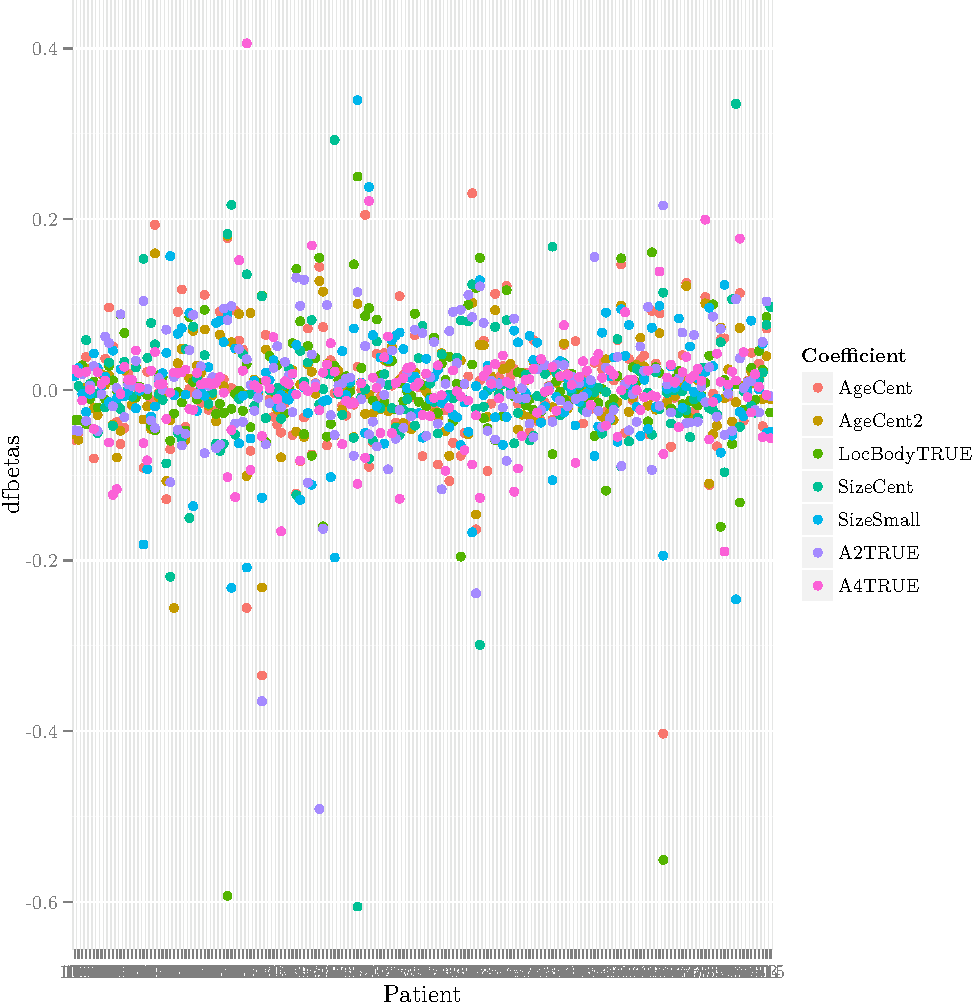
\includegraphics[width=\maxwidth]{figure/05-eda-dfbetas-full-1} 

}



\end{knitrout}
There is quite a number of rather influential observations.  These could do with some checking, but first collapse down the model -- there's little point doing dfbeta fucking about based on coefficients that will never get fit in the end anyway.


\subsection{EDA: Variable selection}
\begin{knitrout}
\definecolor{shadecolor}{rgb}{0.969, 0.969, 0.969}\color{fgcolor}\begin{kframe}
\begin{alltt}
\hlstd{nobs.coxph} \hlkwb{<<-} \hlkwa{function}\hlstd{(}\hlkwc{obj}\hlstd{,} \hlkwc{...}\hlstd{)} \hlkwd{sum}\hlstd{(obj}\hlopt{$}\hlstd{y[,}\hlnum{2}\hlstd{])}
\hlcom{# Note: Exhaustive search at level 2 is only feasible for at most 5 variables}
\hlcom{#fit.cph.as = glmulti(Surv(Time, DSD) ~ strata(SexM) + AgeCent + AgeCent2 + LocBody + SizeCent + SizeSmall + A2 + A4, data = data, marginality = TRUE, method = "h", fitfunction = "coxph", crit = "bic", level = 2)}
\hlkwd{set.seed}\hlstd{(}\hlnum{20150110}\hlstd{)}
\hlstd{fit.cph.as} \hlkwb{=} \hlkwd{glmulti}\hlstd{(}\hlkwd{Surv}\hlstd{(Time, DSD)} \hlopt{~} \hlkwd{strata}\hlstd{(SexM)} \hlopt{+} \hlstd{AgeCent} \hlopt{+} \hlstd{AgeCent2} \hlopt{+} \hlstd{LocBody} \hlopt{+} \hlstd{SizeCent} \hlopt{+} \hlstd{SizeSmall} \hlopt{+} \hlstd{A2} \hlopt{+} \hlstd{A4,} \hlkwc{data} \hlstd{= data,} \hlkwc{marginality} \hlstd{=} \hlnum{TRUE}\hlstd{,} \hlkwc{method} \hlstd{=} \hlstr{"g"}\hlstd{,} \hlkwc{fitfunction} \hlstd{=} \hlstr{"coxph"}\hlstd{,} \hlkwc{crit} \hlstd{=} \hlstr{"bic"}\hlstd{,} \hlkwc{level} \hlstd{=} \hlnum{2}\hlstd{,} \hlkwc{plotty} \hlstd{=} \hlnum{FALSE}\hlstd{,} \hlkwc{report} \hlstd{=} \hlnum{FALSE}\hlstd{)}
\end{alltt}
\begin{verbatim}
## TASK: Genetic algorithm in the candidate set.
## Initialization...
## Algorithm started...
\end{verbatim}


{\ttfamily\noindent\color{warningcolor}{\#\# Warning in fitter(X, Y, strats, offset, init, control, weights = weights, : Loglik converged before variable\ \ 18 ; beta may be infinite.}}\begin{verbatim}
## Improvements in best and average IC have bebingo en below the specified goals.
## Algorithm is declared to have converged.
## Completed.
\end{verbatim}
\begin{alltt}
\hlcom{# fit.cph.as}
\hlcom{# After 830 generations:}
\hlcom{# Best model: Surv(Time,DSD)~1+strata(SexM)+SizeCent+A2+A4}
\hlcom{# Crit= 1367.16344569113}
\hlcom{# Mean crit= 1401.37248769175}
\hlcom{# Improvements in best and average IC have bebingo en below the specified goals.}
\hlcom{# Algorithm is declared to have converged.}
\hlcom{# Completed.}
\hlkwd{rm}\hlstd{(nobs.coxph)}
\end{alltt}
\end{kframe}
\end{knitrout}

Also run BIC stepwise, because we can.
\begin{knitrout}
\definecolor{shadecolor}{rgb}{0.969, 0.969, 0.969}\color{fgcolor}\begin{kframe}
\begin{alltt}
\hlkwd{stepAIC}\hlstd{(fit.cph,} \hlkwc{k} \hlstd{=} \hlkwd{log}\hlstd{(}\hlkwd{nrow}\hlstd{(data)))}
\end{alltt}
\begin{verbatim}
## Start:  AIC=1386
## Surv(Time, DSD) ~ strata(SexM) + AgeCent + AgeCent2 + LocBody + 
##     SizeCent + SizeSmall + A2 + A4
## 
##             Df  AIC
## - AgeCent    1 1381
## - LocBody    1 1381
## - SizeSmall  1 1381
## - AgeCent2   1 1382
## - SizeCent   1 1385
## <none>         1386
## - A4         1 1387
## - A2         1 1388
## 
## Step:  AIC=1381
## Surv(Time, DSD) ~ strata(SexM) + AgeCent2 + LocBody + SizeCent + 
##     SizeSmall + A2 + A4
## 
##             Df  AIC
## - LocBody    1 1376
## - SizeSmall  1 1376
## - AgeCent2   1 1377
## - SizeCent   1 1379
## <none>         1381
## - A4         1 1382
## - A2         1 1383
## 
## Step:  AIC=1376
## Surv(Time, DSD) ~ strata(SexM) + AgeCent2 + SizeCent + SizeSmall + 
##     A2 + A4
## 
##             Df  AIC
## - SizeSmall  1 1371
## - AgeCent2   1 1372
## - SizeCent   1 1375
## <none>         1376
## - A4         1 1377
## - A2         1 1379
## 
## Step:  AIC=1371
## Surv(Time, DSD) ~ strata(SexM) + AgeCent2 + SizeCent + A2 + A4
## 
##            Df  AIC
## - AgeCent2  1 1367
## <none>        1371
## - SizeCent  1 1371
## - A4        1 1372
## - A2        1 1374
## 
## Step:  AIC=1367
## Surv(Time, DSD) ~ strata(SexM) + SizeCent + A2 + A4
## 
##            Df  AIC
## <none>        1367
## - A4        1 1368
## - SizeCent  1 1368
## - A2        1 1370
## Call:
## coxph(formula = Surv(Time, DSD) ~ strata(SexM) + SizeCent + A2 + 
##     A4, data = data)
## 
## 
##            coef exp(coef) se(coef)    z      p
## SizeCent 0.0139      1.01  0.00563 2.47 0.0140
## A2TRUE   0.5845      1.79  0.19894 2.94 0.0033
## A4TRUE   0.4311      1.54  0.18733 2.30 0.0210
## 
## Likelihood ratio test=25.7  on 3 df, p=1.08e-05  n= 196, number of events= 188
\end{verbatim}
\end{kframe}
\end{knitrout}
Consensus, excellent.


\subsection{PH assumption: reduced model}












































